%!TEX root = ../../main.tex
\chapter{Results}\label{chap:results}
\partialtoc

In this chapter, we will review the results for the calculation of the nonlinear
susceptibility, $\boldsymbol{\chi}$, and the SSHG yield,
$\mathcal{R}_{\mathrm{iF}}$, for the the Si(001)(2$\times$1) and the
Si(111)(1$\times$1):H surfaces. These results are the direct product of all the
theory derived in Chapters \ref{chap:chi2} and \ref{chap:sshgyield}. These
example surfaces provide the perfect testbed for the theory developed in this
work, and the resulting spectra yield insight into the various key aspects of
the theory.

The first part focuses on using the Si(001)(2$\times$1) surface to review and
compare the enhancements that we have added to the framework for calculating
$\boldsymbol{\chi}$. This surface is presented in a special configuration that
allows us to test each improvement made on the theory; namely, the use of the
cut function for extracting the surface susceptibility, the effect of the
scissors operator, and the addition of $\boldsymbol{\mathcal{V}}^{\mathrm{nl}}$.
I will also present a very brief overview of the calculated SSHG yield, but with
no comparison to experimental data as there is very little available for this
surface.

The second part features the Si(111)(1$\times$1):H, which is experimentally
well-characterized, and thus provides an excellent platform with which to test
our robust formulation for the SSHG yield. We will first compare the calculated
$\chi^{xxx}$ component with experimental data from Ref. \cite{hoferAPA96}. This
will provide a nice confirmation of everything we learned from the
Si(001)(2$\times$1) surface. We will then review the calculated spectra for
different polarization cases of the incoming fields, and compare them to
experimental data from Refs. \cite{bergfeldPRL04, mejiaPRB02, mitchellSS01},
over a wide energy range covering both the E$_{1}$ and E$_{2}$ critical point
transitions for bulk Si. We will find that this new formalism, that is developed
from the 3-layer model and includes the effect of multiple reflections in the
material, compares quite favorably with the experimental data. The quality of
these calculations affords us some insight into how the SSHG spectrum can
affected by several physical factors.


%%%%%%%%%%%%%%%%%%%%%%%%%%%%%%%%%%%%%%%%%%%%%%%%%%%%%%%%%%%%%%%%%%%%%%%%%%%%%%%%
%%%%%%%%%%%%%%%%%%%%%%%%%%%%%%%%%%%%%%%%%%%%%%%%%%%%%%%%%%%%%%%%%%%%%%%%%%%%%%%%

\section{Results for the \texorpdfstring{Si(001)(2$\times$1)}{Si(001)(2x1)}
surface}\label{sec:Si2x1results}

In this section, let us review the characteristics of the Si(001)(2$\times$1)
surface we will be using for the subsequent calculations. This surface provides
an excellent test case to check the consistency of our approach for calculating
$\boldsymbol{\chi}$ with the new elements described in Chap. \ref{chap:chi2}.
For this, I have selected a clean Si(001) surface with a 2$\times$1 surface
reconstruction. The slab for such a surface could be made centrosymmetric by
creating the front and back surfaces with the same 2$\times$1 reconstruction.
However, this particular slab has the lower surface terminated with hydrogen,
producing a terminated, ``ideal'' bulk Si surface. The H atoms saturate the
dangling bonds of the bulk-like Si atoms at the surface, as seen in Fig.
\ref{fig:2x1struc}. Consider the $z$ coordinate pointing out of the surface with
the $x$ coordinate along the crystallographic [011] direction, parallel to the
dimers.

\begin{figure}[t]
\centering
\subbottom[Front view.\label{fig:2x1front}]%
{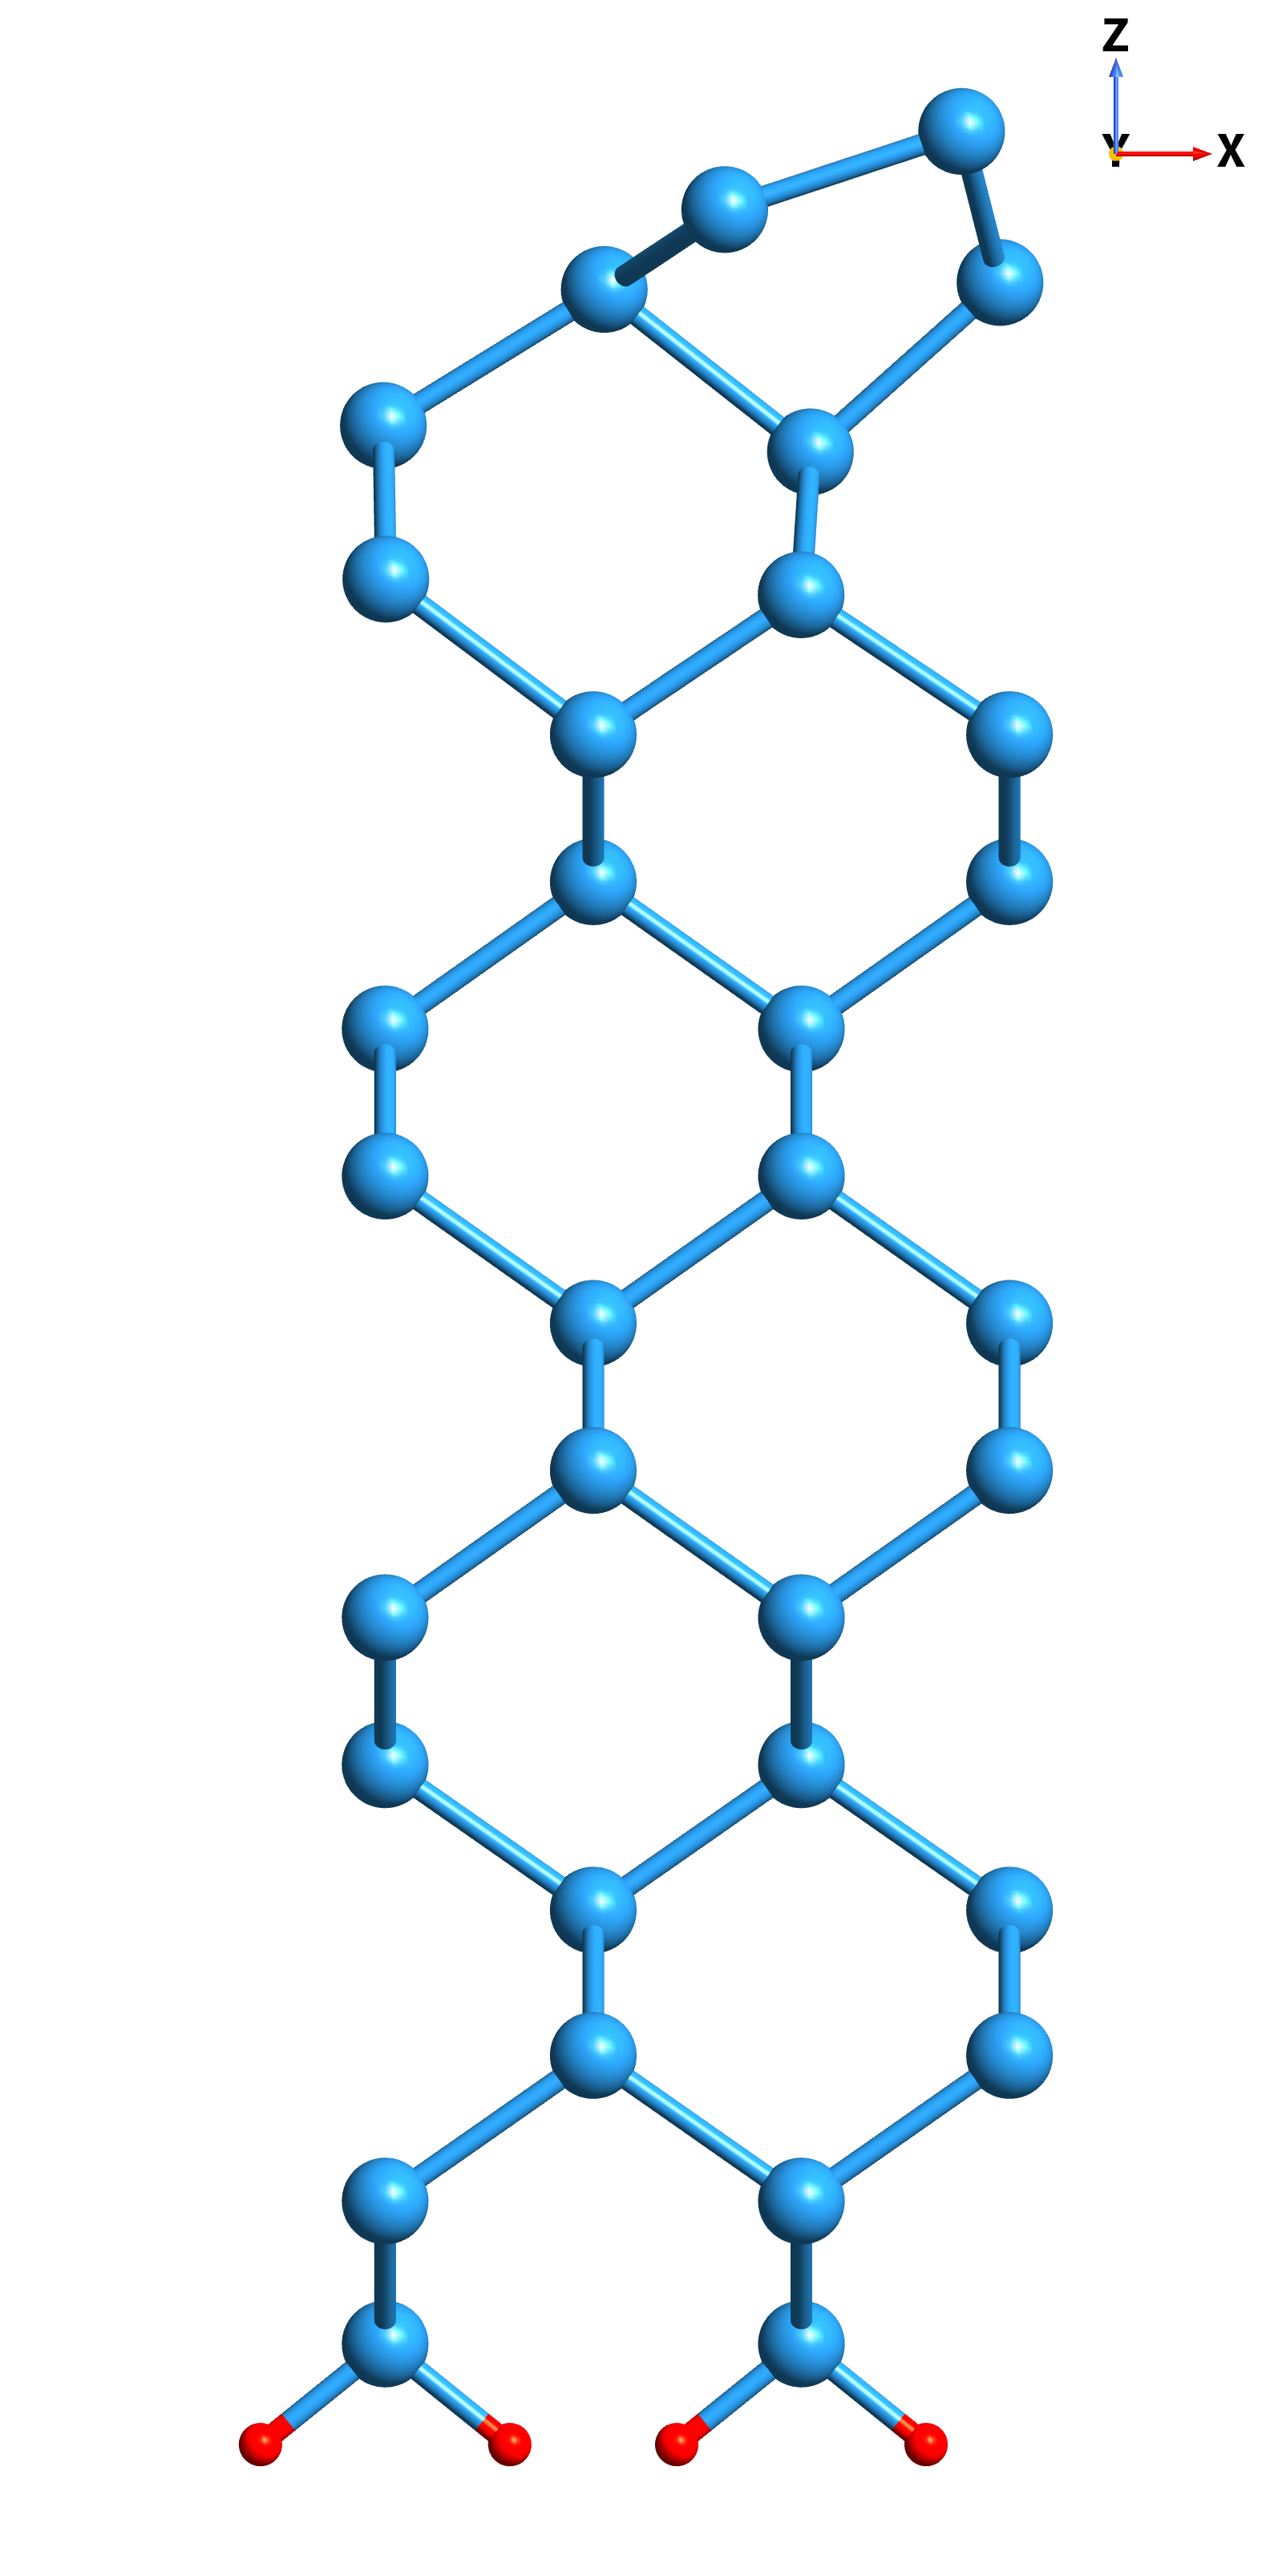
\includegraphics[width=0.3\textwidth]{content/figures/struc-Si2x1-front}}\hfill
\subbottom[Side view.\label{fig:2x1side}]%
{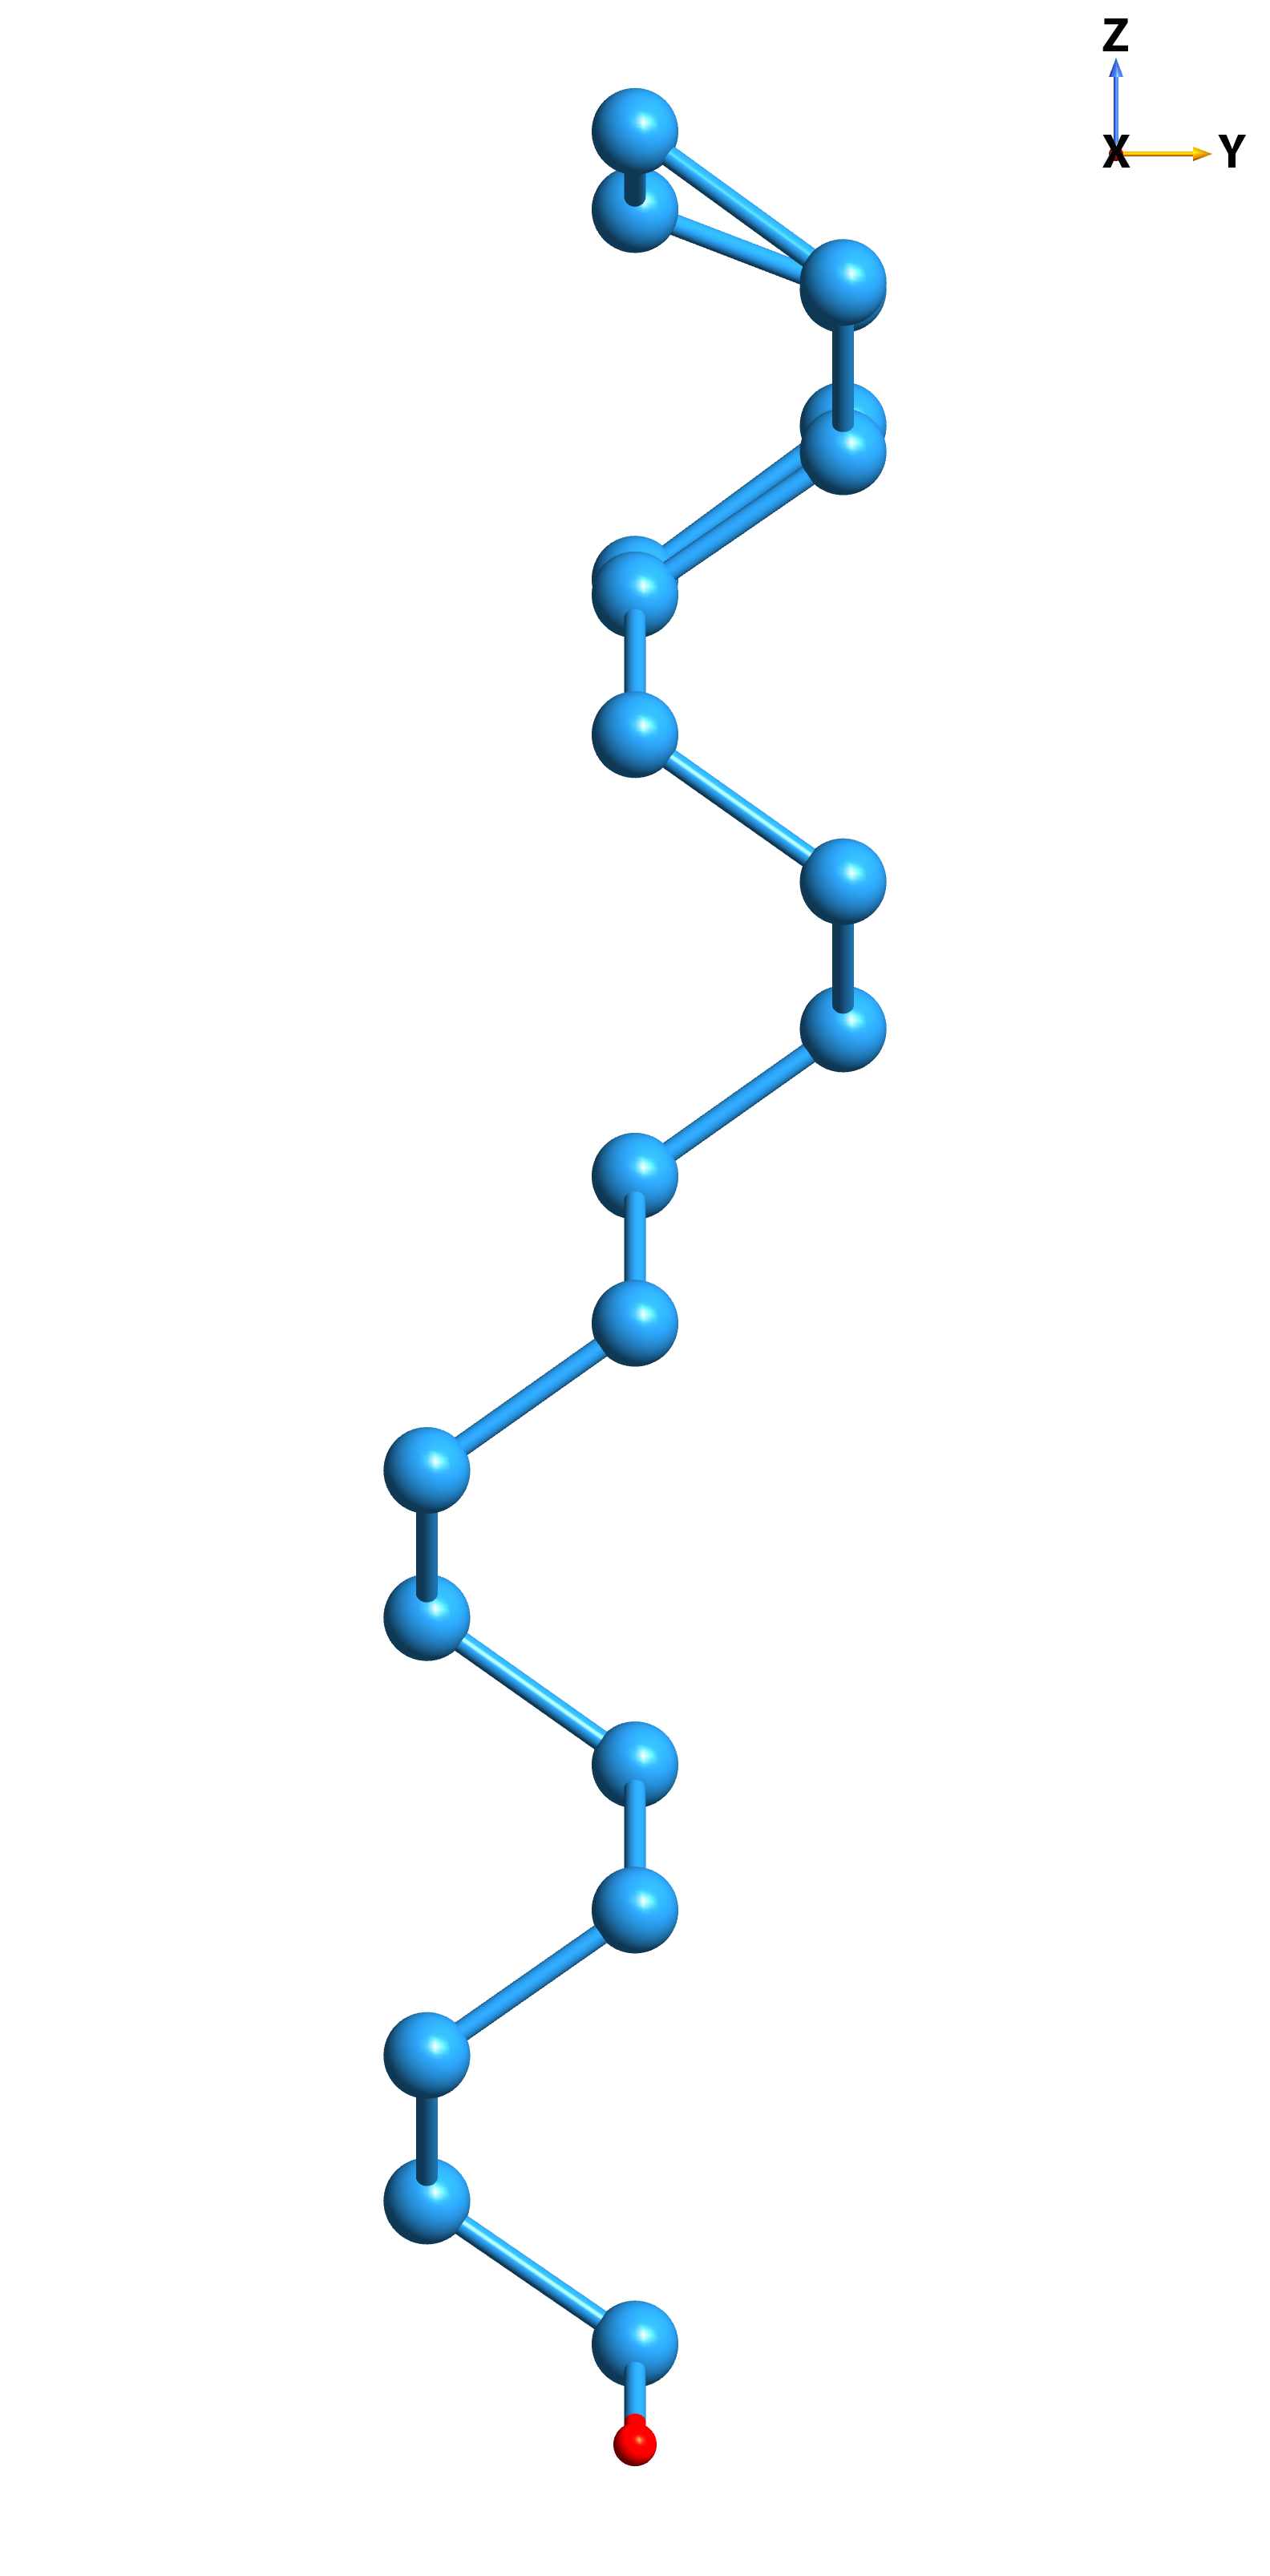
\includegraphics[width=0.3\textwidth]{content/figures/struc-Si2x1-side}}\hfill
\subbottom[Top view.\label{fig:2x1top}]%
{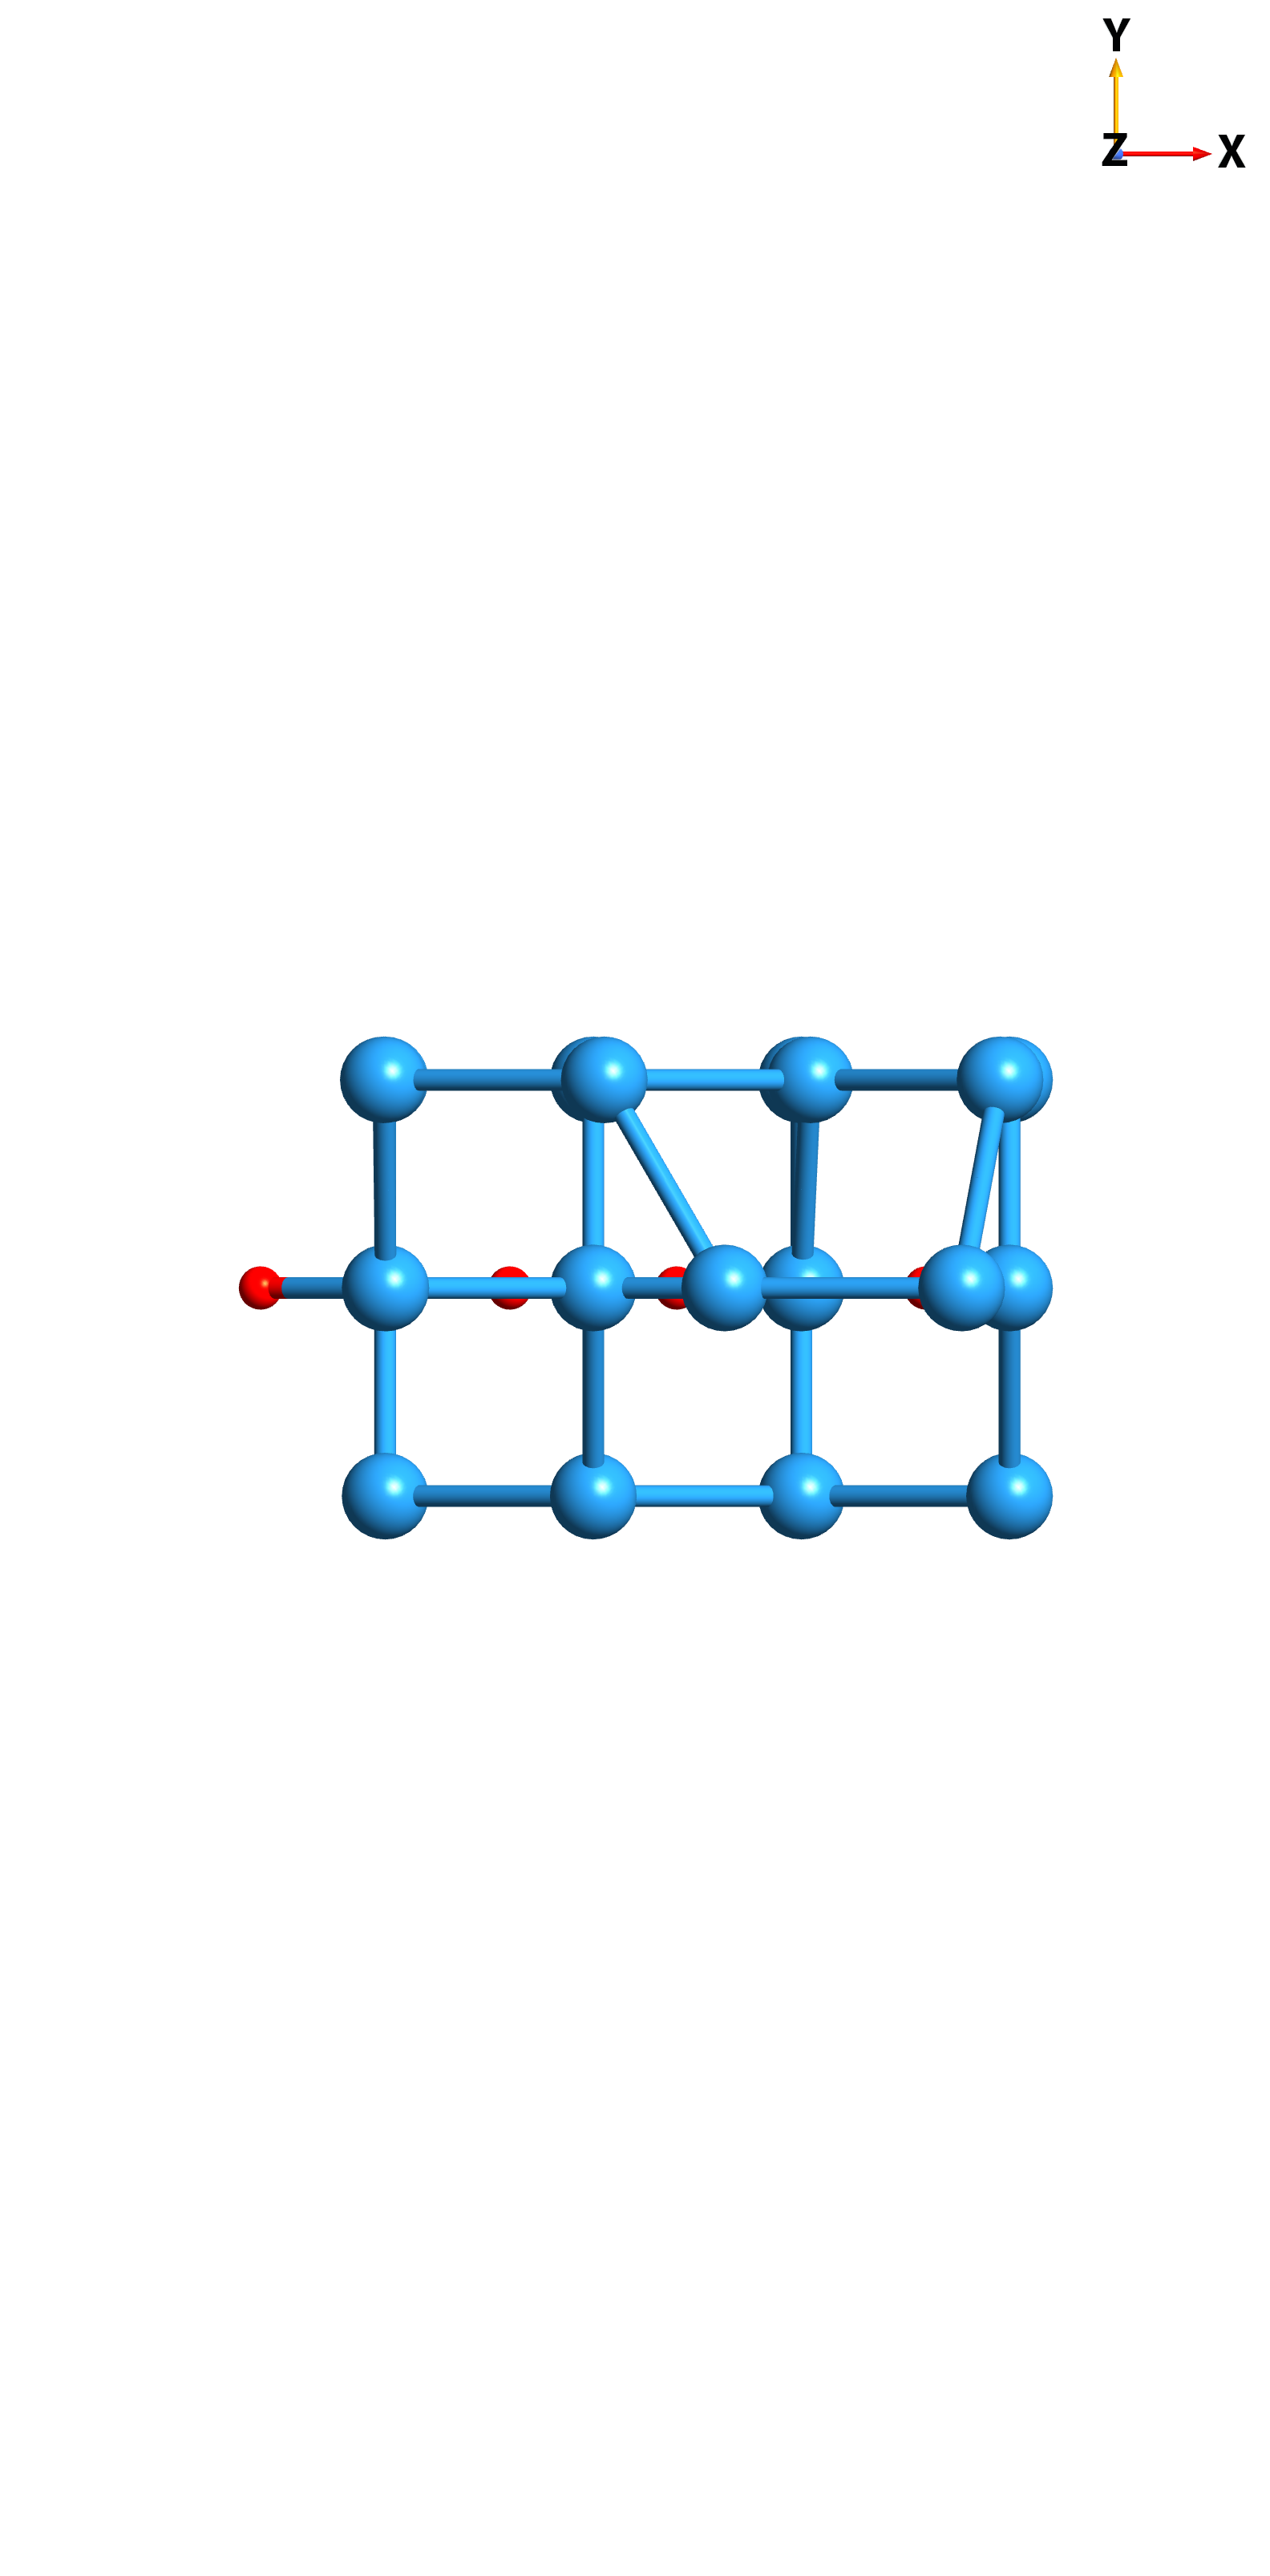
\includegraphics[width=0.3\textwidth]{content/figures/struc-Si2x1-top}}
\caption{Several views of the slab used to represent the Si(001)(2$\times$1)
surface. This particular slab has 16 Si atomic layers (large blue balls) with
two H atomic layers (small red balls).}
\label{fig:2x1struc}
\end{figure}

The self-consistent ground state and the Kohn-Sham states were calculated in the
DFT-LDA framework using the plane-wave ABINIT code \cite{gonzeCPS09, abinit},
using Troullier-Martins pseudopotentials \cite{troullierPRB91} that are fully
separable nonlocal pseudopotentials in the Kleinman-Bylander form
\cite{kleinmanPRL82}. The contribution of $\mathbf{v}^\mathrm{nl}$ and
$\boldsymbol{\mathcal{V}}^\mathrm{nl}$ to Eq. \eqref{eq:chis} was carried out
using the DP code \cite{olevanoDP}.

The surface was studied with the experimental lattice constant of 5.43 \AA.
Structural optimizations were also performed with the ABINIT code. The geometry
optimization was carried out in slabs of 12 atomic layers, where the central
four layers where fixed at the bulk positions. The structures were relaxed until
the Cartesian force components were less than 5 meV/\AA. The geometry
optimization for the clean surface gives a dimer buckling of 0.721 \AA, and a
dimer length of 2.301 \AA. For the dihydride surface, the obtained Si-H bond
distance was 1.48 \AA. These results are in good agreement with previous
theoretical studies \cite{caramellaPRB09, mendozaPRB06}. The vacuum size is
equivalent to one quarter the size of the slab, avoiding the effects produced by
possible wave-function tunneling from the contiguous surfaces of the full
crystal formed by the repeated super-cell scheme \cite{mendozaPRB06}.

Spin-orbit, local field, and electron-hole attraction \cite{beyond} effects on
the SHG process are all neglected. Although these are important factors in the
optical response of a semiconductor, their efficient calculation is still
theoretically and numerically challenging and under debate. This merits further
study but is beyond the scope of this thesis. For a given slab size, I found the
converged spectra to obtain the relevant parameters. The most important of these
are: an energy cutoff of 10 Ha for the 16, 24, and 32 layered slabs and 13 Ha
for the 40 layer slab, an equal number of conduction and valence bands, and a
set of 244 \textbf{k} points in the irreducible Brillouin zone, which are
equivalent to 1058 \textbf{k} points when disregarding symmetry relations. The
\textbf{k} points are used for the linear analytic tetrahedron method for
evaluating the 3D Brillouin Zone (BZ) integrals, where special care was taken to
examine the double resonances of Eq. \eqref{eq:chis} \cite{nastosPRB05}. Note
that the Brillouin zone for the slab geometry collapses to a 2D-zone, with only
one $\mathbf{k}$-point along the $z$-axis.

{\color{red}
$T^{\mathrm{a}\mathrm{b}}_{nm}=(i/\hbar)
[r^\mathrm{b},v^{\mathrm{nl},\mathrm{a}}]_{nm}$ must be evaluated in order to
obtain Eqs. \eqref{tau.1} and \eqref{tau.1n} that are required for Eq.
\eqref{eq:chis}. Computing second-order derivatives is necessary, making the
numerical procedure very time consuming. This adds significantly to the already
lengthy time needed for the calculation of the $\mathbf{v}^\mathrm{nl}$
contribution that is proportional only to the first-order derivatives. Memory
requirements are also greatly increased for both $\mathbf{v}^\mathrm{nl}$ and
$[\mathbf{r},\mathbf{v}^\mathrm{nl}]$. However, the contribution from
$[\mathbf{r},\mathbf{v}^\mathrm{nl}]$ is very small \cite{valerie} and it is
therefore neglected in this work.}


%%%%%%%%%%%%%%%%%%%%%%%%%%%%%%%%%%%%%%%%%%%%%%%%%%%%%%%%%%%%%%%%%%%%%%%%%%%%%%%%

\subsection{Calculating \texorpdfstring{$\chi^{xxx}$}{Xxxx}}
\label{sec:res2x1chi}

The idea behind the special slab configuration, pictured in Fig.
\ref{fig:si2x1slab}, is that the crystalline symmetry of the H terminated
surface imposes that $\chi_{\mathrm{H}}^{xxx}=0$. The 2$\times$1 surface has no
such restrictions, so naturally $\chi_{2\times 1}^{xxx}\ne 0$. This is due to
the fact that along the $y$ direction there is a mirror plane for the
H-saturated surface (causing centrosymmetry), whereas for the 2$\times$1 surface
this mirror is lost as the dimers are asymmetric along $x$. Thus, calculating
$\chi^{xxx}$ for the full-slab, or the upper half-slab containing the 2$\times$1
surface \cite{note1} should yield the same result, since the contribution from
the H saturated surface is zero regardless. The following relationship must be
satisfied for this particular slab,
\begin{equation*}
\chi_{\mathrm{half-slab}}^{xxx} =
\chi_{\mathrm{full-slab}}^{xxx},
\end{equation*}
where $\chi_{\mathrm{half-slab}}^{xxx}$ is calculated using
${\mathbf{\mathcal{C}}}(z) = 1$ for the upper half containing the 2$\times$1
surface reconstruction (see Fig. \ref{fig:si2x1slab}), and
$\chi_{\mathrm{full-slab}}^{xxx}$ is calculated using ${\mathbf{\mathcal{C}}}(z)
= 1$ for the entire slab. Again, the dihydride surface on the lower half of the
slab must have $\chi_{\mathrm{half-slab}}^{xxx} = 0$.

\begin{figure}[t]
\centering 
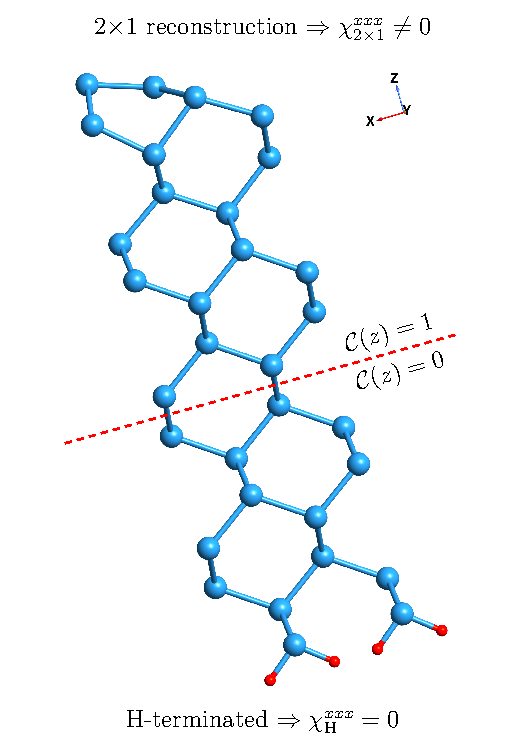
\includegraphics[width=0.45\textwidth]{content/figures/struc-Si2x1-rot}
\caption{The slab for the Si(001)(2$\times$1) surface. The front (upper) surface
is in a 2$\times$1, clean reconstruction, and the rear (lower) surfaces is
H-terminated, with ``ideal'' bulk-like atomic positions. The dangling bonds are
H-saturated.}
\label{fig:si2x1slab}
\end{figure} 

Note that all spectra for $\chi^{xxx}$ presented in this section were calculated
with a Gaussian broadening of 0.15 eV.


%%%%%%%%%%%%%%%%%%%%%%%%%%%%%%%%%%%%%%%%%%%%%%%%%%%%%%%%%%%%%%%%%%%%%%%%%%%%%%%%

\subsubsection{Full-slab results}\label{sec:fsresults}

Fig. \ref{fig:layersconv} shows $|\chi_{\mathrm{full-slab}}^{xxx}|$ for the slab
with 16, 24, 32, and 40 Si atomic layers, without the contribution of
$\mathbf{v}^{\mathrm{nl}}$, and with no scissors correction. Since the clean
Si(001) surface is in a 2$\times$1 reconstruction there are two atoms per atomic
layer. Thus, the total number of atoms per slab is twice the number of atomic
layers of the slab. The slabs were extended in the $z$ directions in steps of 8
layers of bulk-like atomic positions. Note that the response differs
substantially for 16 and 24 layers but is quite similar for 32 and 40 layers. As
explained above, the calculation of the $\mathbf{v}^\mathrm{nl}$ contribution is
computationally expensive, so it is crucial to minimize the number of atoms in
the calculation. I consider a slab with 32 Si atomic layers as a good compromise
between the convergence of $\chi^{xxx}_{\mathrm{full-slab}}$ as a function of
the number of layers in the slab, and the computational expense.

\begin{figure}[b]
\centering 
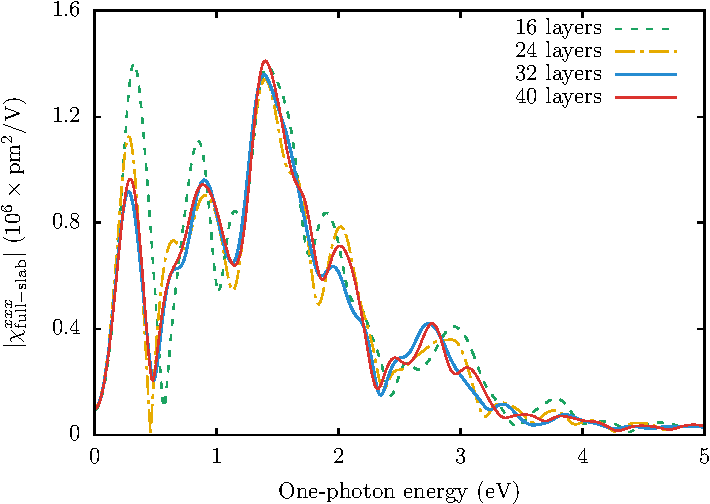
\includegraphics[width=0.6\textwidth]{content/figures/fig-Si2x1-layerconv}
\caption{$\vert\chi_{\mathrm{full-slab}}^{xxx}\vert$ vs $\hbar\omega$ for the
slab with 16, 24, 32, and 40 atomic Si layers. Adequate convergence is achieved
after 32 layers. The spectra presented here do not include the contribution from
$\mathbf{v}^{\mathrm{nl}}$, with a scissors value of $\hbar\Delta = 0$ eV.}
\label{fig:layersconv}
\end{figure}


%%%%%%%%%%%%%%%%%%%%%%%%%%%%%%%%%%%%%%%%%%%%%%%%%%%%%%%%%%%%%%%%%%%%%%%%%%%%%%%%

\subsubsection{Half-slab vs full-slab}

Now that we have established an adequate number of layers to attain convergence,
we can proceed to study the spectra produced from the slab with 32 atomic
layers. Fig. \ref{fig:hsvfs} presents a comparison between
$\chi^{xxx}_{\mathrm{half-slab}}$ and $\chi^{xxx}_{\mathrm{full-slab}}$ for four
different scenarios: with and without the effects of $\mathbf{v}^\mathrm{nl}$,
and with two values for the scissors correction, $\hbar\Delta$. I have chosen a
scissors value of $\hbar\Delta=0.5$ eV, that is the GW gap reported in Refs.
\cite{rohlfingPRB95, garciaCPC01}. This is justified by the fact that the
surface states from the clean 2$\times$1 surface are rigidly shifted and
maintain their dispersion relation with respect to the LDA value, according to
the GW calculations of Ref.
\cite{rohlfingPRB95}.

We can appreciate that the difference between the half-slab and full-slab
responses is quite small for all four scenarios. Indeed, when the value
$\vert\chi^{xxx}\vert$ is large, the difference between the two is quite small;
when $\vert\chi^{xxx}\vert$ is small, the difference increases slightly but the
spectra is so close to zero that it is negligible. Of course, the difference
between the two would decrease as the number of atomic layers increases. Note
how 32 layers in the slab is more than enough to confirm that the extraction of
the surface second-harmonic susceptibility from the 2$\times$1 surface is
readily possible using the formalism contained in Eq. \eqref{eq:chis}.
Calculating the response from the lower half of the slab substantiates that
$\vert\chi^{xxx}_{\mathrm{half-slab}}\vert\approx 0$ for the dihydride surface
(not shown).

This confirms the validity of the theory developed in \ref{chap:chi2} and is an
important result of this work. Through the proposed layer formalism, we can
calculate the surface $\chi^{\mathrm{abc}}$ component including the contribution
from the nonlocal part of the pseudopotentials, and part of the many-body
effects through the scissors correction. Therefore, this scheme is robust and
versatile and should work for any crystalline surface.

\begin{figure}[H]
\centering 
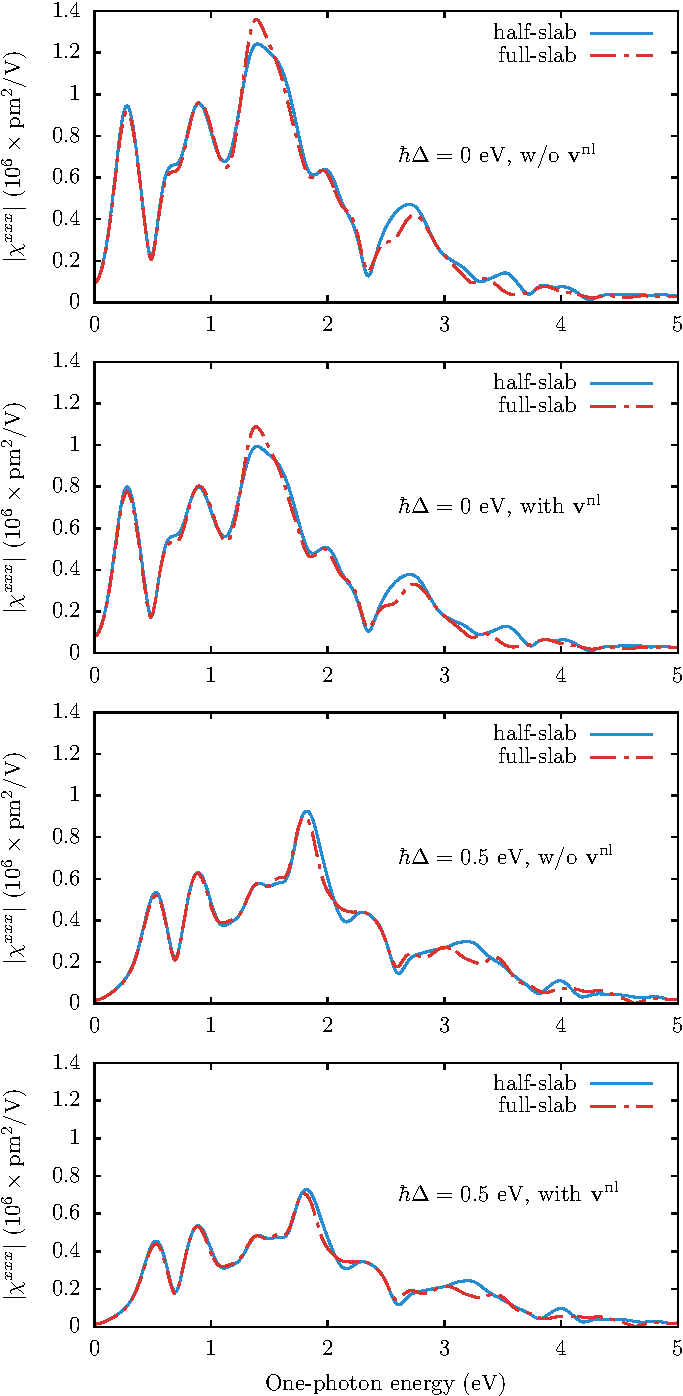
\includegraphics[height=0.9\textheight]{content/figures/fig-Si2x1-hsvsfs}
\caption{$\chi^{xxx}_{\mathrm{half-slab}}$ and $\chi^{xxx}_{\mathrm{full-slab}}$
vs $\hbar\omega$ for four different combinations: with and without the effects
of $\mathbf{v}^\mathrm{nl}$, and with two values for the scissors correction,
$\hbar\Delta$.}
\label{fig:hsvfs}
\end{figure}


%%%%%%%%%%%%%%%%%%%%%%%%%%%%%%%%%%%%%%%%%%%%%%%%%%%%%%%%%%%%%%%%%%%%%%%%%%%%%%%%

\subsubsection{Half-slab results}

I proceed to explain some of the features seen in
$\vert\chi^{xxx}_{\mathrm{half-slab}}\vert$ that is obtained when setting
$\mathbf{\mathcal{C}}(z) = 1$ for the upper half containing the 2$\times$1
surface reconstruction, as seen in Fig. \ref{fig:si2x1slab}. From Fig.
\ref{fig:hsvfs}, we note a series of resonances that derive from the $1\omega$
and $2\omega$ terms in Eq. \eqref{eq:chis}. Notice that the $2\omega$ resonances
start below $E_{g}/2$, where $E_{g}$ is the band gap (0.53 eV for LDA, and 1.03
eV if the scissor is used with $\hbar\Delta=0.5$ eV). These resonances come from
the electronic states of the 2$\times$1 surface, that lie inside the bulk band
gap of Si and are the well known electronic surface states \cite{rohlfingPRB95}.

Fig. \ref{fig:vnl} shows that the inclusion of $\mathbf{v}^\mathrm{nl}$ reduces
the value of $\vert\chi^{xxx}_{\mathrm{half-slab}}\vert$ by 15-20\%. This
demonstrates the importance of this contribution for a fully correct SSHG
calculation. This is in agreement with the analysis for bulk semiconductors
\cite{luppiPRB08}. However, the inclusion of $\mathbf{v}^\mathrm{nl}$ does not
change the spectral shape of $\vert\chi^{xxx}_{\mathrm{half-slab}}\vert$. We can
confirm that this is not unique for this specific scissors shift, as we can
appreciate from the upper two panels of Fig. \ref{fig:hsvfs}, with $\hbar\Delta
= 0$ eV.

\begin{figure}[H]
\centering 
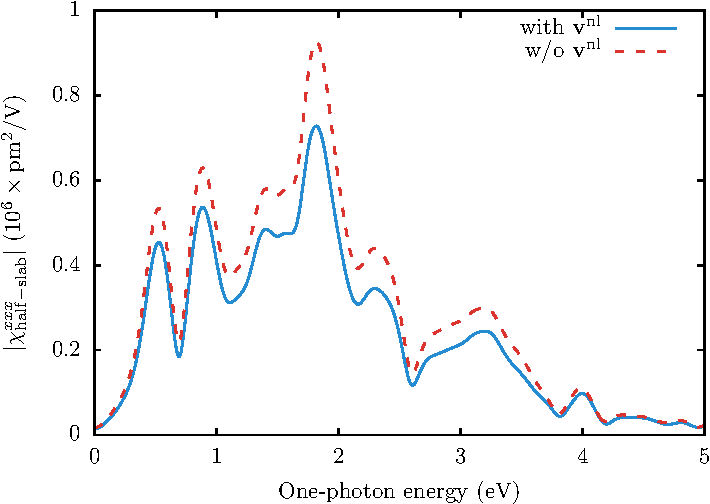
\includegraphics[width=0.6\textwidth]{content/figures/fig-Si2x1-vnl}
\caption{$\chi^{xxx}_{\mathrm{half-slab}}$ vs $\hbar\omega$, with and without
the contribution from $\mathbf{v}^\mathrm{nl}$. This spectrum has a scissors
value of $\hbar\Delta=0.5$ eV.}
\label{fig:vnl}
\end{figure}

To demonstrate the effect of the scissors correction, I considered two different
finite values for $\hbar\Delta$. The first, with a value of $\hbar\Delta=0.5$ eV
that is used in the previous results, is the ``average'' GW gap taken from Ref.
\cite{rohlfingPRB95} that is in agreement with Ref. \cite{garciaCPC01}. The
second, with a value of $\hbar\Delta=0.63$ eV is the ``average'' gap taken from
Ref. \cite{asahiPRB00}, where more \textbf{k} points in the Brillouin zone were
used to calculate the GW value. Fig. \ref{fig:scissors} shows that the scissors
correction shifts the spectra from its LDA value to higher energies, as
expected. However, contrary to the case of linear optics \cite{cabellosPRB09},
the shift introduced by the scissors correction is not rigid, which is
consistent with the work of Ref. \cite{nastosPRB05}. This is because the
second-harmonic optical response mixes $1\omega$ and $2\omega$ transitions (see
Eq. \eqref{eq:chis}), and accounts for the non-rigid shift. The reduction of the
spectral strength is in agreement with previous calculations for bulk systems
\cite{nastosPRB05, luppiPRB10, leitsmannPRB05}.

When comparing $\vert\chi^{xxx}_{\mathrm{half-slab}}\vert$ for the two finite
values of $\hbar\Delta$, it is clear that the first two peaks are almost rigidly
shifted with a small difference in height while the rest of the peaks are
modified substantially. This behavior comes from the fact that the first two
peaks are almost exclusively related to the $2\omega$ resonances of Eq.
\eqref{eq:chis}. The other peaks are a combination of $1\omega$ and $2\omega$
resonances and yield a more varied spectrum. Note that for large-gap materials
the $1\omega$ and $2\omega$ resonances would be split, producing a small
interference effect. The $2\omega$ resonances would still strongly depend on the
surface states. Thus, small changes in the scissors shift can affect the SSH
susceptibility spectrum quite dramatically. In Ref. \cite{adolphPRB00}, the
authors already noted that the nonlinear optical response of bulk materials is
more influenced by the electronic structure of the material than the linear
case. For the case of semiconductor surfaces, the problem is even more intricate
due to the presence of electronic surface states.

\begin{figure}[H]
\centering 
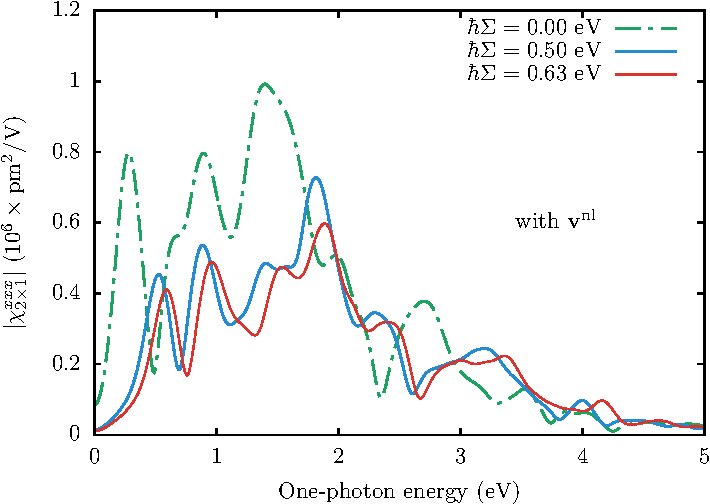
\includegraphics[width=0.5\textwidth]{content/figures/fig-Si2x1-scissors}
\caption{$\chi^{xxx}_{\mathrm{half-slab}}$ vs $\hbar\omega$ for a slab with 32
atomic Si layers plus one H layer, for three different values of the scissors
correction, $\hbar\Delta$.
\label{fig:scissors}} 
\end{figure}

The high sensitivity of SSHG to the energy position of surface states, as seen
in Fig. \ref{fig:scissors}, makes SSHG a good benchmark tool for
spectroscopically testing the validity of the inclusion of many-body effects,
and in particular the quasi-particle correction to the electronic states.
Although local fields are neglected, in principle they should be quite small
parallel to the interface as the electric field is continuous. $\chi^{xxx}$
should have a relatively small influence from these local fields. Excitonic
effects should also be explored, but their efficient calculation is
theoretically and numerically challenging \cite{beyond} and far beyond the scope
of this work. Unfortunately the experimental measurement of the $\chi^{xxx}$
component is difficult as the SH radiated intensity would be proportional not
only to this component but also to the other components of $\boldsymbol{\chi}$.
However, I will present this exact comparison later on in Sec.
\ref{sec:res1x1chi} for the Si(111)(1$\times$1):H surface.


%%%%%%%%%%%%%%%%%%%%%%%%%%%%%%%%%%%%%%%%%%%%%%%%%%%%%%%%%%%%%%%%%%%%%%%%%%%%%%%%

\subsection{Overview of the calculated \texorpdfstring{$\mathcal{R}$}{R}
spectra}\label{sec:2x1R3D}

In Figs. \ref{fig:2x1rP3d} and \ref{fig:2x1rS3d}, I present the results for the
calculation of the SSHG yield for our test surface. The 2$\times$1 surface
reconstruction yields a Class 1, primitive triclinic system with all 18
components independent from each other \cite{popovbook}. We cannot take
advantage of any symmetry relations for this surface. However, this is no
problem for the robust formulation we derived in Chapter \ref{chap:sshgyield}
that can accommodate all 18 components disregarding any surface symmetries.
Calculating all 18 components is obviously more time consuming, but they can be
efficiently parallelized so very little time is actually lost.

\begin{figure}[h]
\centering
\subbottom[$\mathcal{R}_{pP}$\label{fig:2x1rpp3d}]%
{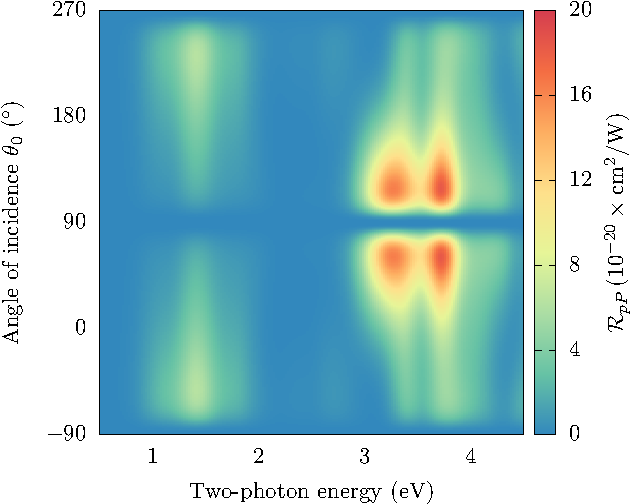
\includegraphics[height=0.4\textwidth]{content/figures/3D-Si2x1-RpP.pdf}}\hfill
\subbottom[$\mathcal{R}_{sP}$\label{fig:2x1rsp3d}]%
{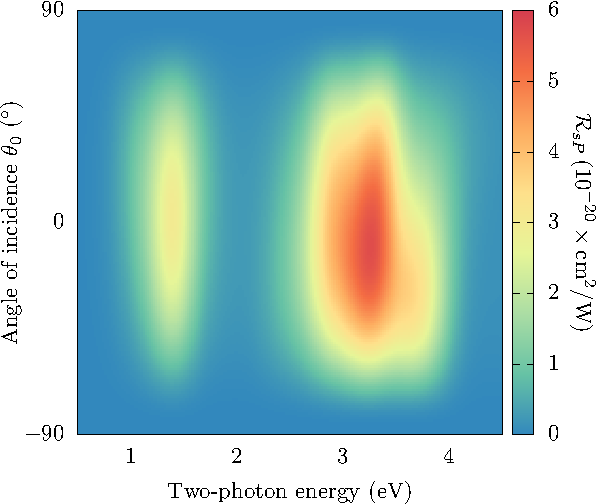
\includegraphics[height=0.4\textwidth]{content/figures/3D-Si2x1-RsP.pdf}}
\caption{$\mathcal{R}$ for outgoing $P$ polarization, versus the angle of
incidence ($\theta_{0}$) for the Si(001)(2$\times$1) surface. The scissor shift
used was $\hbar\Delta = 0.5$ eV. Both figures consider an azimuthal angle of
$\phi = 45^{\circ}$. All curves are broadened with $\sigma = 0.10$ eV.}
\label{fig:2x1rP3d}
\end{figure}

Fig. \ref{fig:2x1rP3d} presents the results for the SSHG yield with outgoing $P$
polarization. I set a fixed azimuthal angle of $\phi = 45^{\circ}$ and then
varied the incoming angle $\theta_{0}$ from $-90^{\circ}$ to $270^{\circ}$. We
can clearly see that the surface states associated with the 2$\times$1
reconstruction produce significant intensity between 1-2 eV in the two-photon
energy range. This is consistent with the findings presented in the previous
section and in Ref. \cite{andersonPRB15}. The intensity of the peak related to
the surface states is significantly lower than the peaks produced in the 2.5-4
eV two-photon energy range. Overall peak intensity is quite high for this
surface, which is consistent as it is highly non-centrosymmetric. The spectrum
for $\mathcal{R}_{pP}$ is very consistent with other calculations of this type
\cite{tancognedejean:tel-01235611}, and even with some limited experimental data
\cite{powerPRL95}.

\begin{figure}[h]
\centering
\subbottom[$\mathcal{R}_{pS}$\label{fig:2x1rps3d}]%
{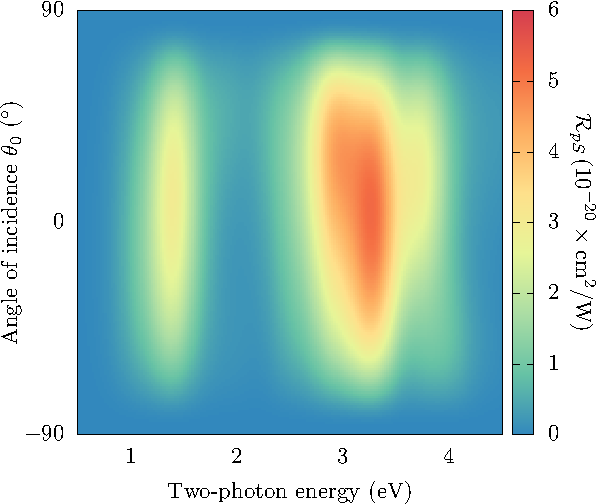
\includegraphics[height=0.4\textwidth]{content/figures/3D-Si2x1-RpS.pdf}}\hfill
\subbottom[$\mathcal{R}_{sS}$\label{fig:2x1rss3d}]%
{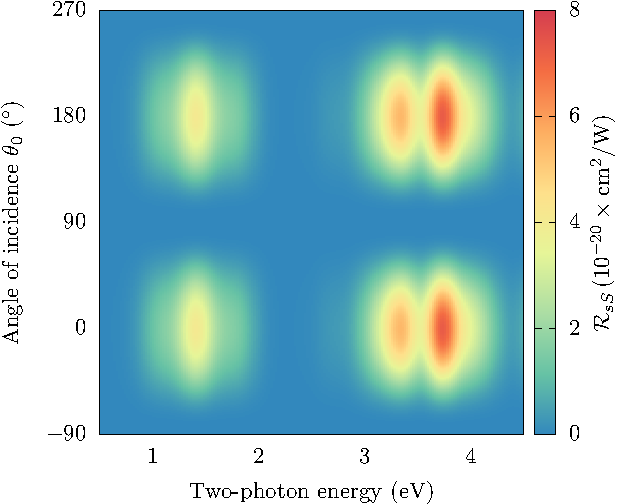
\includegraphics[height=0.4\textwidth]{content/figures/3D-Si2x1-RsS.pdf}}
\caption{$\mathcal{R}$ for outgoing $S$ polarized fields, versus the angle of
incidence ($\theta_{0}$) for the Si(001)(2$\times$1) surface. The scissor shift
used was $\hbar\Delta = 0.5$ eV. Both figures consider an azimuthal angle of
$\phi = 45^{\circ}$. All curves are broadened with $\sigma = 0.10$ eV.}
\label{fig:2x1rS3d}
\end{figure}

Fig. \ref{fig:2x1rS3d} presents the results for the SSHG yield with outgoing $S$
polarization. They are quite similar to what we observed in Fig.
\ref{fig:2x1rP3d}, with a peak related to the surface states between 1-2 eV, and
a larger set of peaks between 2.4-4 eV in the two-photon energy range. These
spectra have a clear maxima around $\theta_{0} = 0^{\circ}$ and $\theta_{0} =
180^{\circ}$.

These plots are presented for mainly illustrative purposes, as there is little
experimental data to compare with the theoretical spectrum. However, these kinds
of plots will be quite useful to the experimentalist interested in this kind of
spectroscopy. Excellent intensity for all polarization cases can be obtained for
small beam angles, such as $\theta_{0} = 30^{\circ}$.


%%%%%%%%%%%%%%%%%%%%%%%%%%%%%%%%%%%%%%%%%%%%%%%%%%%%%%%%%%%%%%%%%%%%%%%%%%%%%%%%
%%%%%%%%%%%%%%%%%%%%%%%%%%%%%%%%%%%%%%%%%%%%%%%%%%%%%%%%%%%%%%%%%%%%%%%%%%%%%%%%

\section{Results for the \texorpdfstring{Si(111)(1$\times$1):H}{Si(111)(1x1):H}
surface}\label{sec:Si1x1results}

We will now focus our attention on the Si(111)(1$\times$1):H surface. This
surface is a $C_{3v}$, primitive hexagonal system with only 4 nonzero components
independent from each other, as shown in Table \ref{tab:chis} \cite{popovbook,
sipePRB87, mizrahiJOSA88}. It is composed of stacked layers with one Si atom
each, with one H atom terminating each surface. The added H saturates the
surface Si dangling bonds and eliminates any surface-related electronic states
in the band gap. Here, the top and bottom surfaces are mirror images (see Fig.
\ref{fig:1x1struc}); this provides the centrosymmetry that necessitates the use
of the cut function to extract the nonzero surface response. In Sec.
\ref{sec:res1x1chi} we will compare the spectrum produced by using relaxed and
unrelaxed coordinates, so it is worth reviewing this concept here. The specifics
of this process are as follows.

The relaxation process was done by my colleague, Nicolas Tancogne-Dejean
\cite{tancognedejean:tel-01235611}. The structure was initially constructed with
the experimental lattice constant of 5.43 \AA, and then performed structural
optimizations with the ABINIT \cite{gonzeCPS09, abinit} code. It was then
relaxed until the Cartesian force components were less than 5 meV/\AA, yielding
a final Si-H bond distance of 1.50 \AA. The energy cutoff used was 20 Ha, and
Troullier-Martin LDA pseudopotentials were used \cite{troullierPRB91}. The
resulting atomic positions are in good agreement with previous theoretical
studies \cite{kaxirasPRB88, jonaPRB95, alfonsoPRB96, cargnoniJOCP00,
mejiaPRB02}, as well as the experimental value for the Si-H distance
\cite{weastCRC88}.

I also evaluated the number of layers required for convergence (like Sec.
\ref{sec:fsresults}) and settled on a slab with 48 atomic Si planes. The
geometric optimizations mentioned above are therefore carried out on slabs of 48
atomic layers without fixing any atoms to the bulk positions. Fig.
\ref{fig:1x1struc} depicts a sample slab with 16 layers of Si. The surface
susceptibilities must be extracted from only half of the slab. This encompasses
24 layers of Si and the single layer of H that terminates the top surface. The
vacuum size is equivalent to one quarter the size of the slab, avoiding the
effects produced by possible wave-function tunneling from the contiguous
surfaces of the full crystal formed by the repeated super-cell scheme
\cite{mendozaPRB06}.

\begin{figure}[H]
\centering
\subbottom[Front view.\label{fig:1x1front}]%
{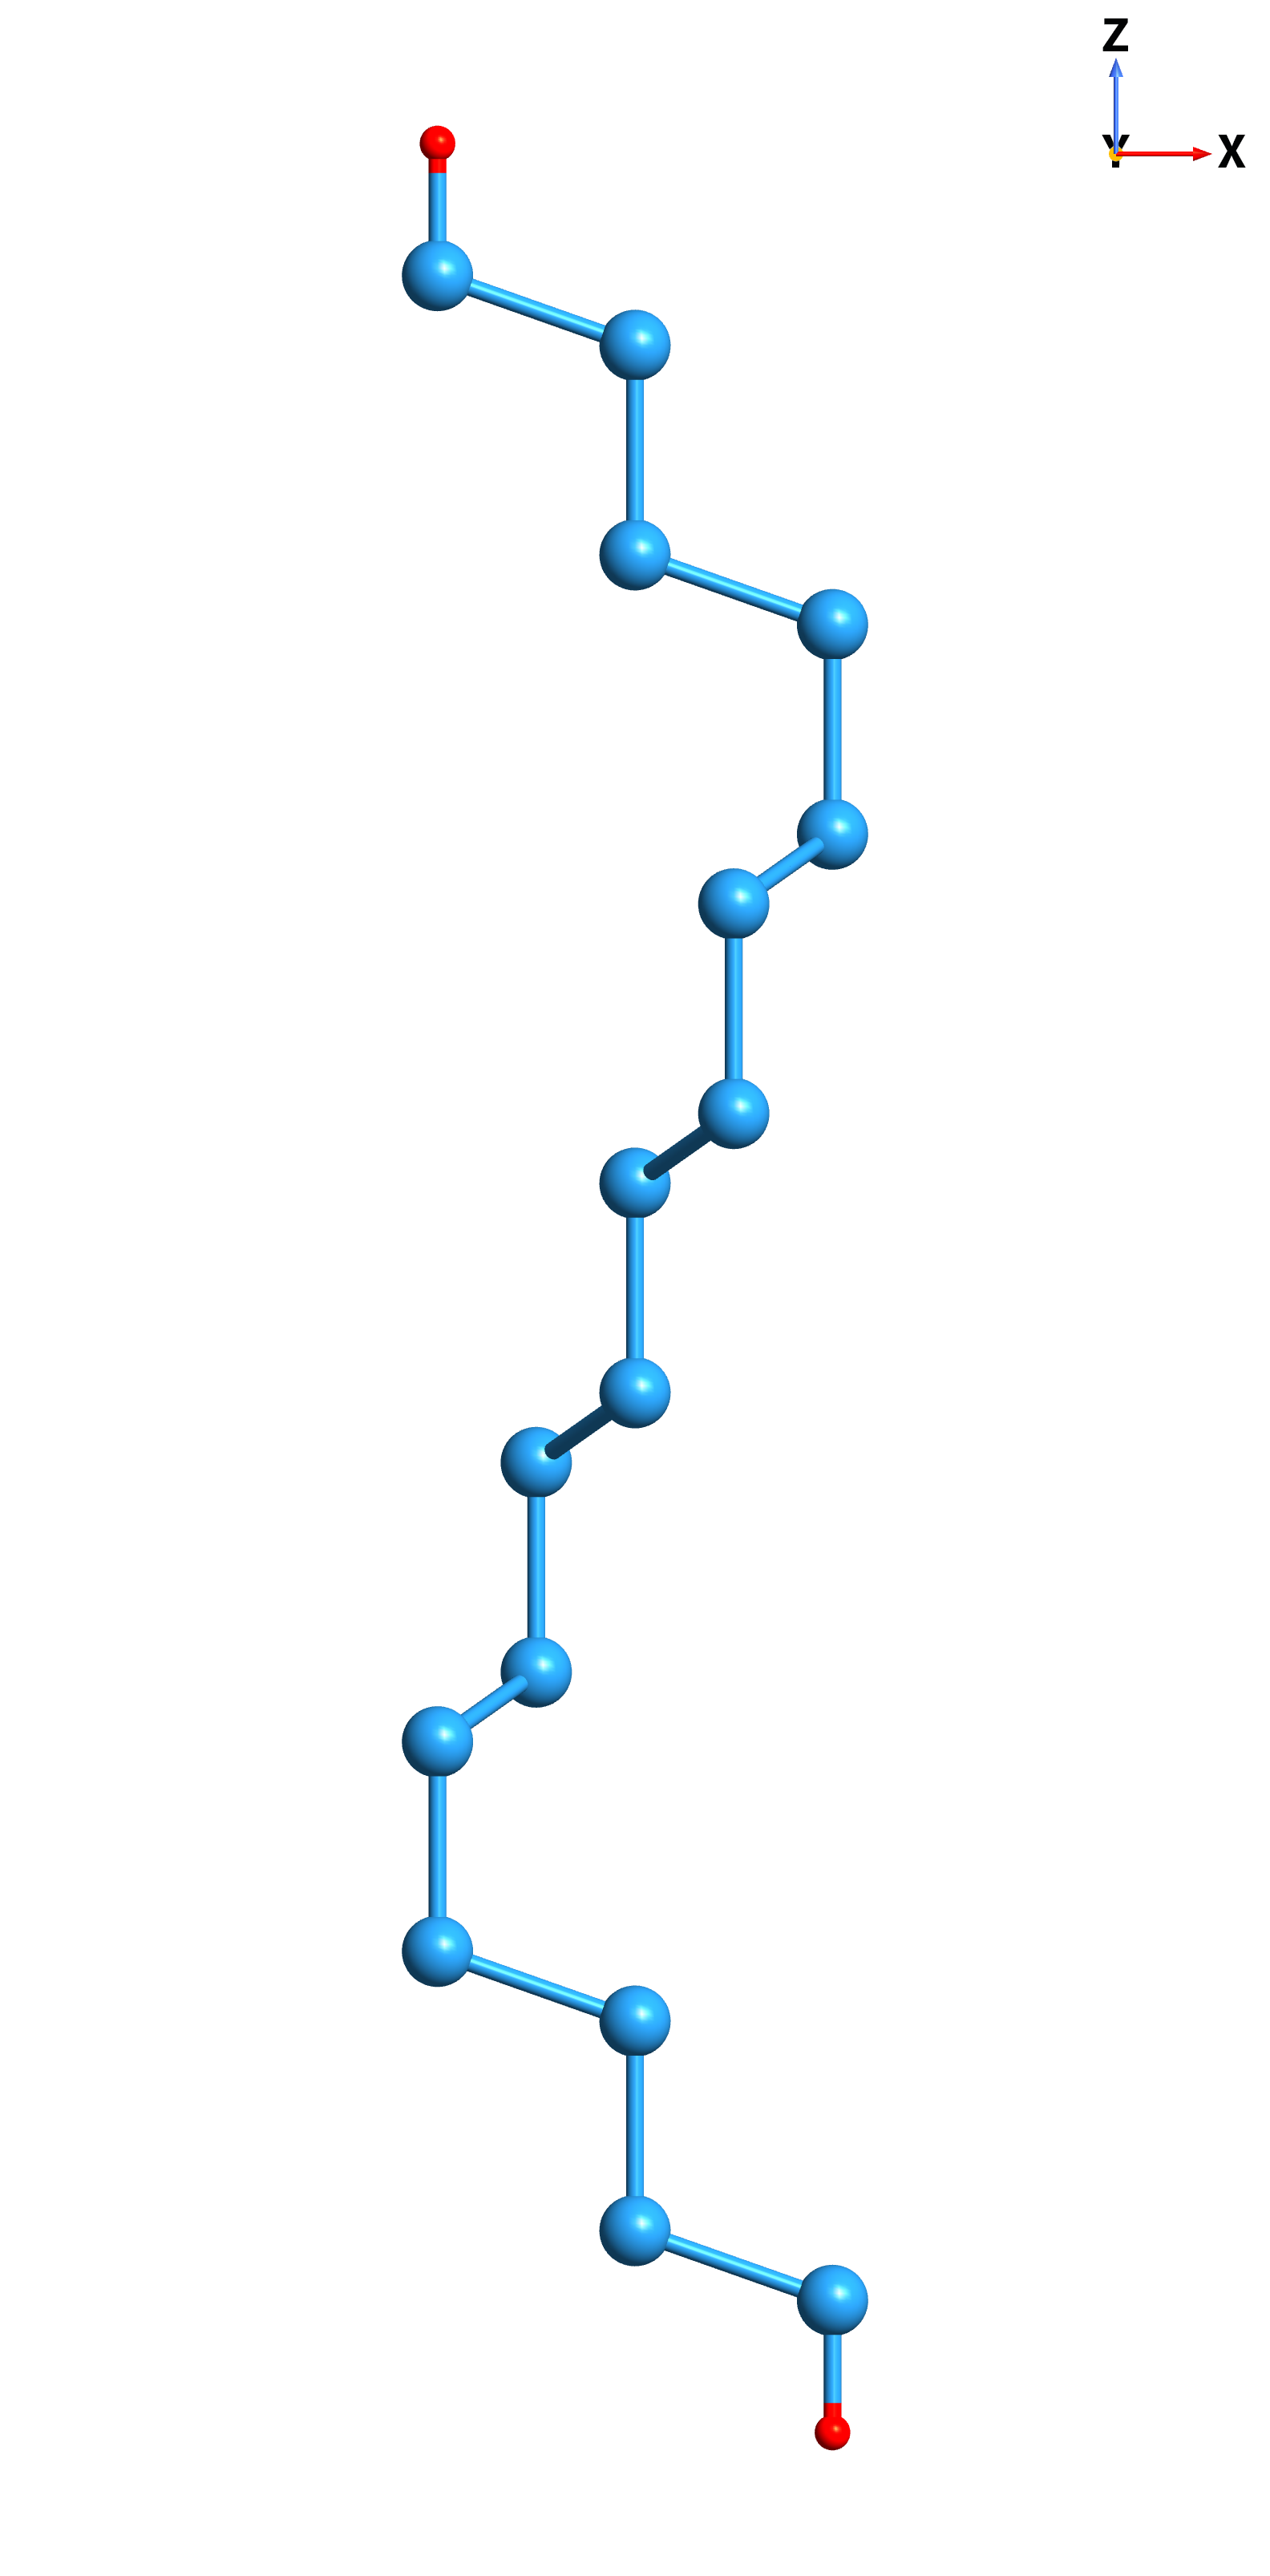
\includegraphics[width=0.3\textwidth]{content/figures/struc-Si1x1-front}}\hfill
\subbottom[Side view.\label{fig:1x1side}]%
{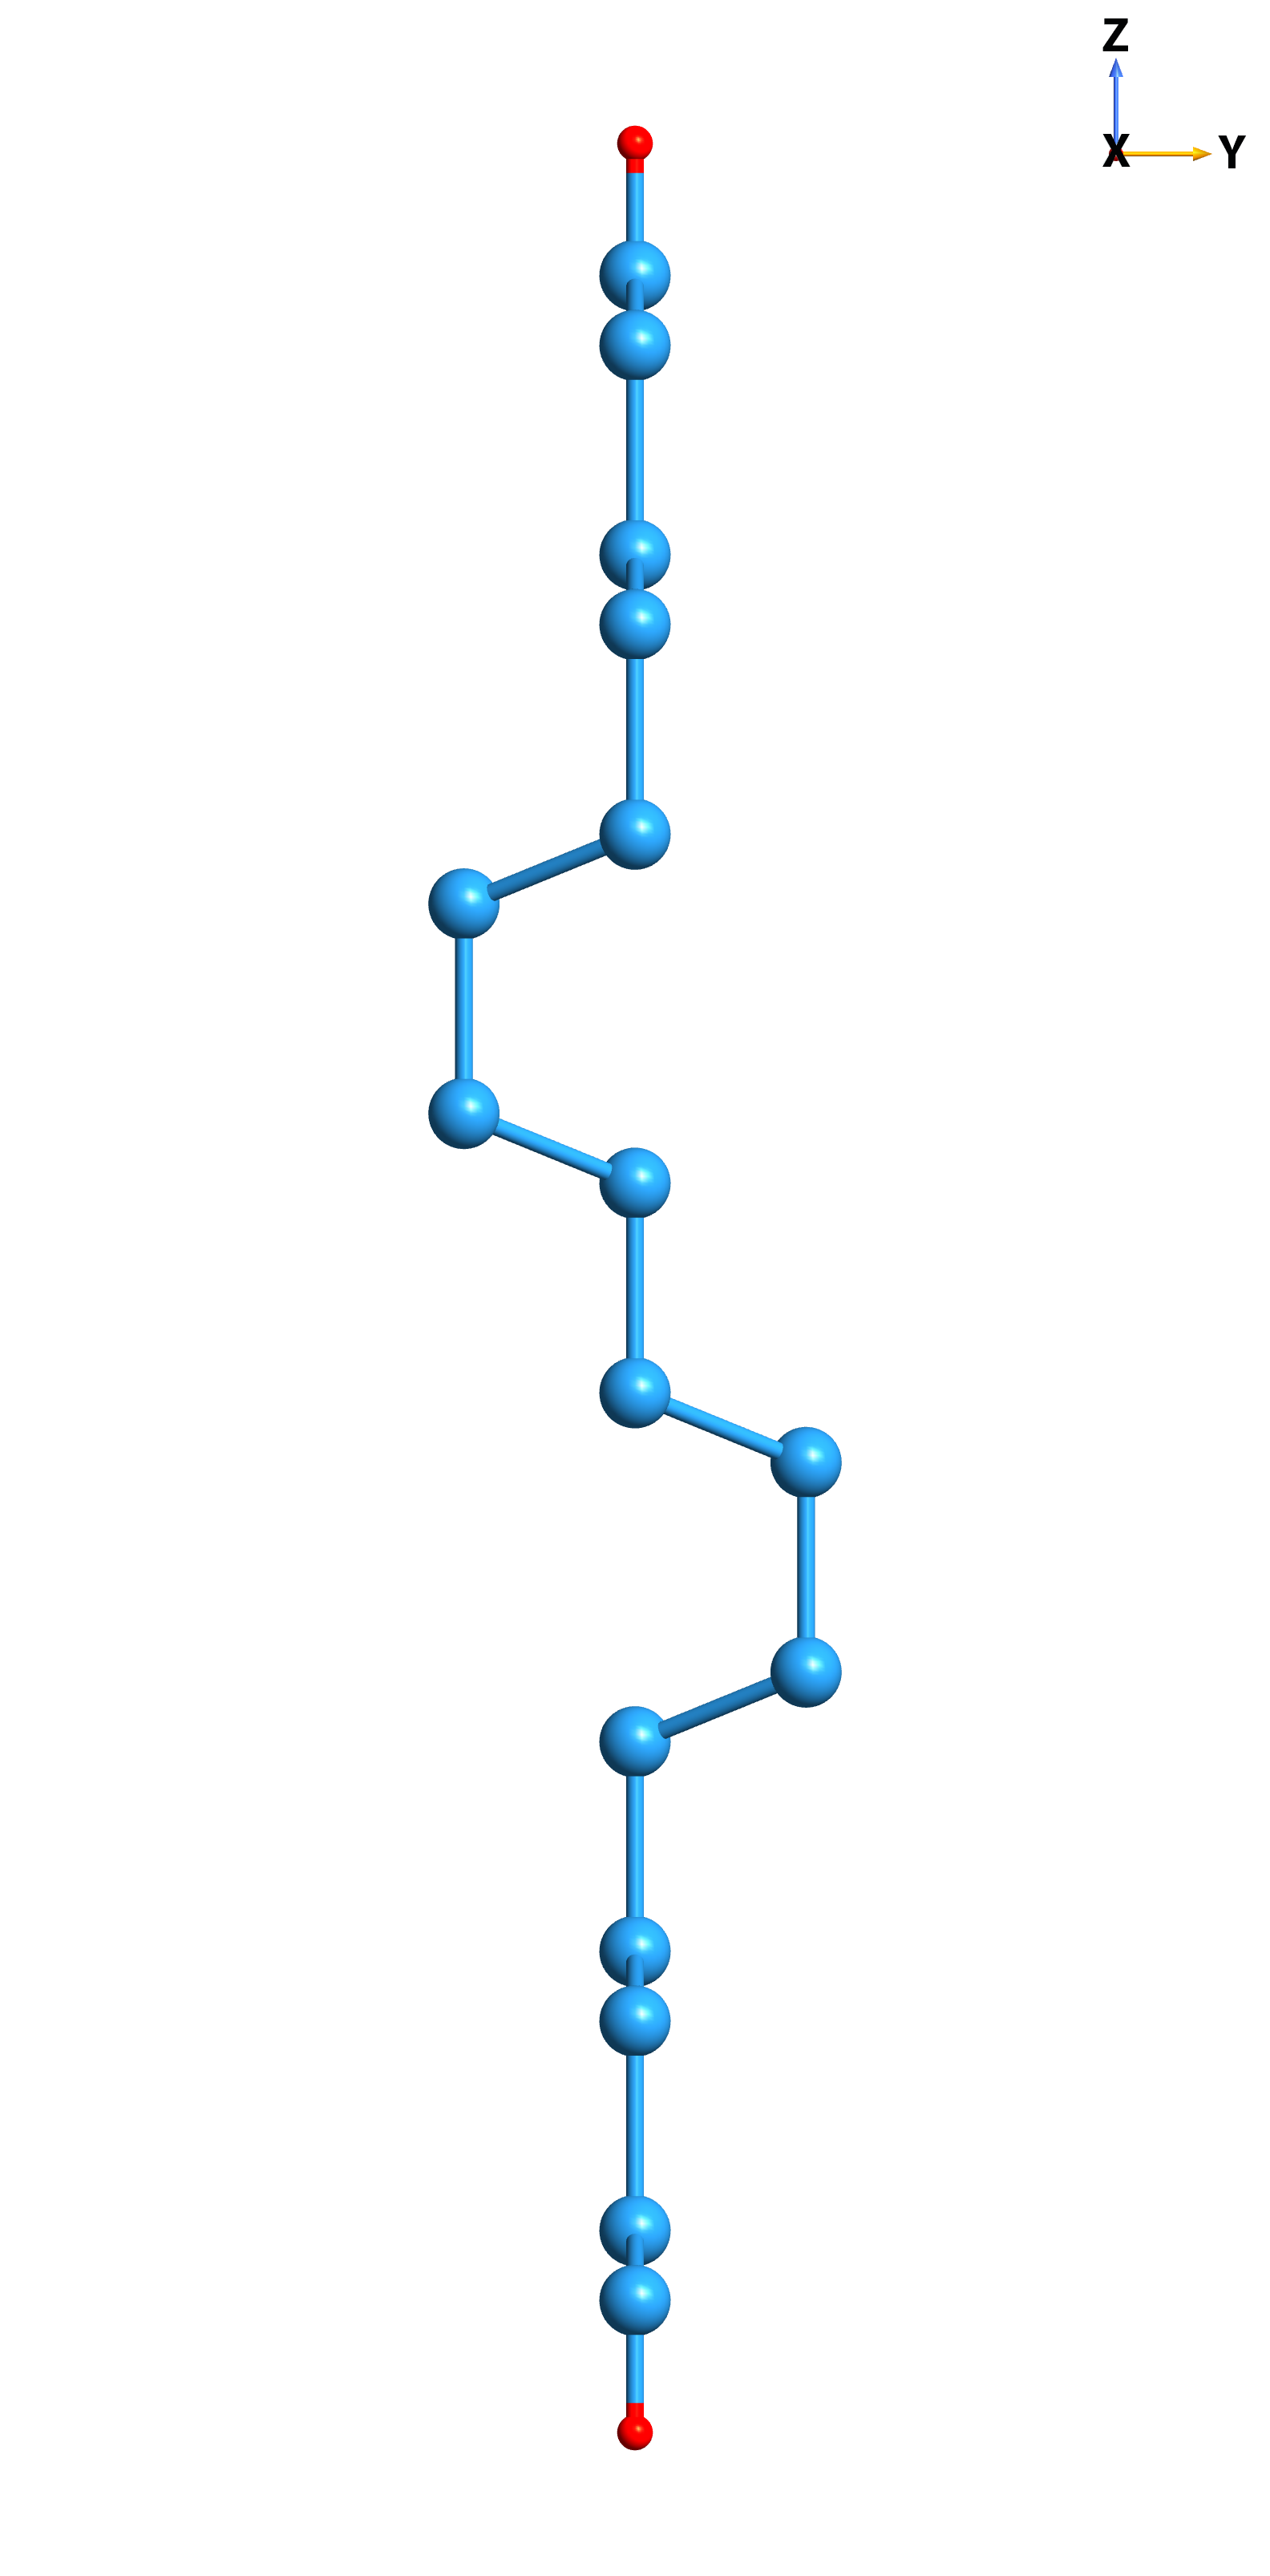
\includegraphics[width=0.3\textwidth]{content/figures/struc-Si1x1-side}}\hfill
\subbottom[Top view.\label{fig:1x1top}]%
{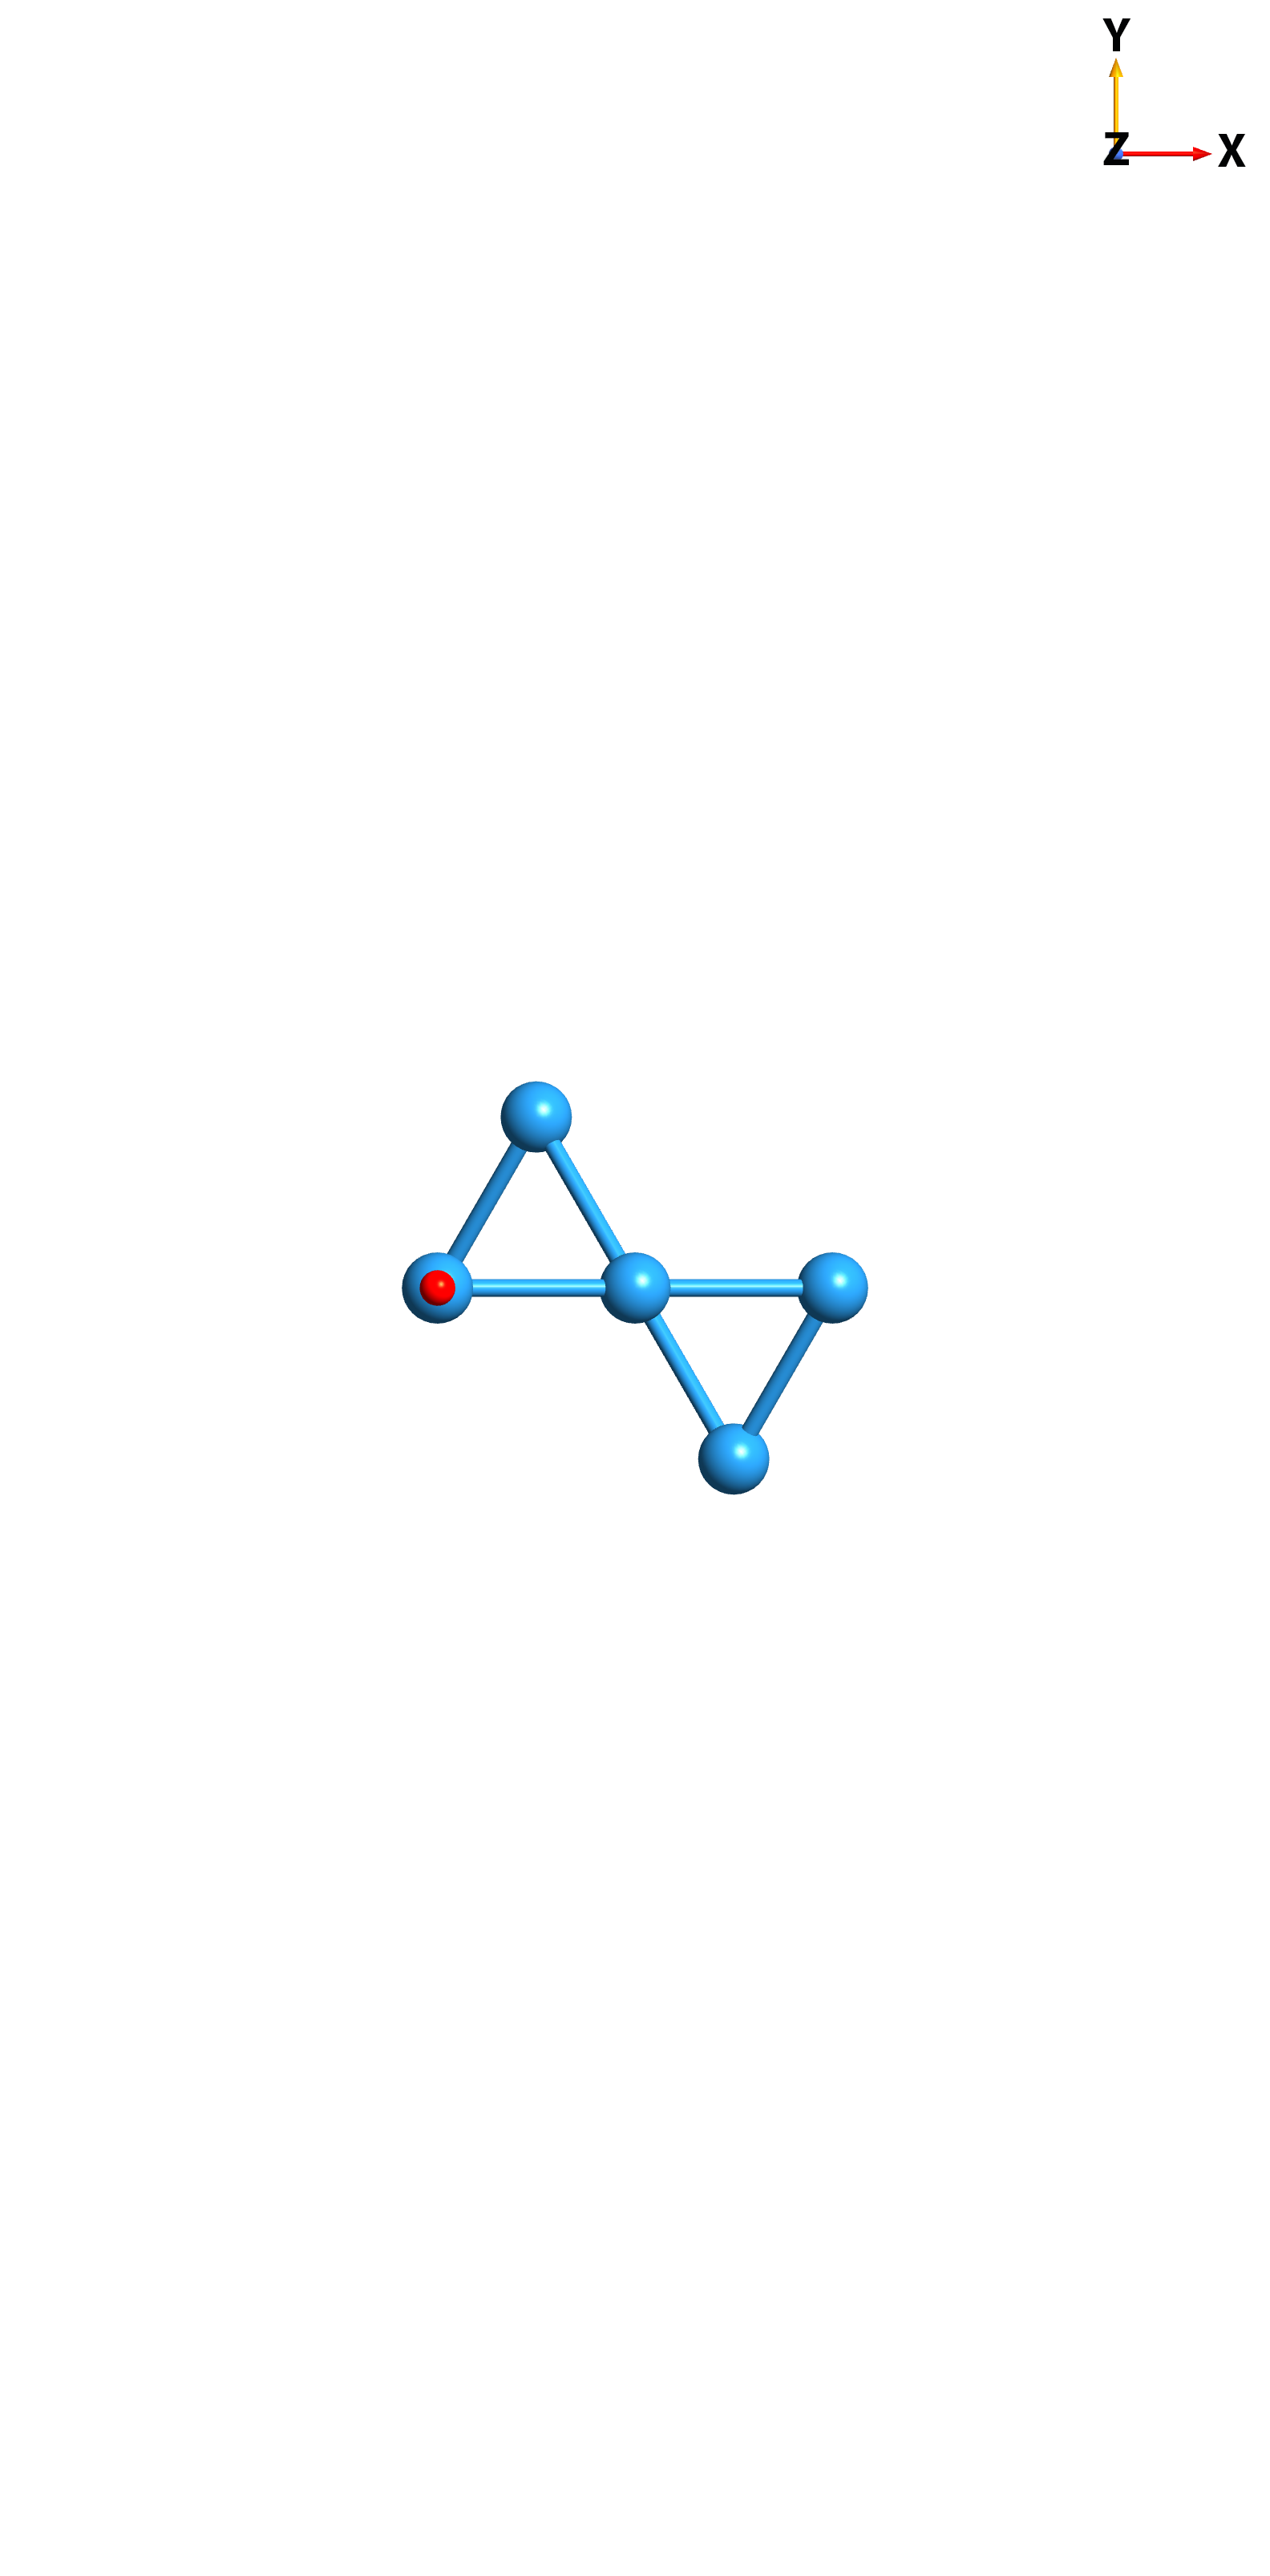
\includegraphics[width=0.3\textwidth]{content/figures/struc-Si1x1-top}}
\caption{Several views of the slab used to represent the Si(111)(1$\times$1):H
surface. This particular slab has 16 Si atomic layers (large blue balls) with
two H atomic layers (small red balls).}
\label{fig:1x1struc}
\end{figure}

The electronic wave-functions, $\psi_{n\mathbf{k}}(\mathbf{r})$, were also
calculated with the ABINIT code using a planewave basis set with an energy
cutoff of 15 Hartrees. $\chi^{\mathrm{abc}}$ was properly converged with 576
\textbf{k} points in the irreducible Brillouin zone, which are equivalent to
1250 \textbf{k} points when disregarding symmetry relations. The contribution of
$\boldsymbol{\mathcal{V}}^\mathrm{nl}$ in Eq. \eqref{eq:chis} was carried out
using the DP\cite{olevanoDP} code with a basis set of 3000 planewaves.
Convergence for the number of bands was achieved at 200, which includes 97
occupied bands and 103 unoccupied bands.

All spectra were produced using a scissors value of 0.7 eV in the
$\chi^{\mathrm{abc}}$ and $\boldsymbol{\epsilon}_{\ell}(\omega)$ calculations.
This value was obtained from Ref. \cite{liPRB10}, in which the authors carry out
a $\mathrm{G}_{0}\mathrm{W}_{0}$ calculation on this surface for increasing
numbers of layers. They calculated the LDA and $\mathrm{G}_{0}\mathrm{W}_{0}$
band gaps, and found that the difference between the two tends towards
$\sim0.7$ eV as more layers are added, culminating in a value of 0.68 eV for
bulk Si. This calculation is completely \emph{ab-initio}, so I consider 0.7 eV
to be a very reasonable value for the scissors correction.


%%%%%%%%%%%%%%%%%%%%%%%%%%%%%%%%%%%%%%%%%%%%%%%%%%%%%%%%%%%%%%%%%%%%%%%%%%%%%%%%

\subsection{Calculating \texorpdfstring{$\chi^{xxx}$}{Xxxx}}
\label{sec:res1x1chi}

The pioneering work presented in Ref. \cite{mejiaPRB02} showed the effect of
artificially moving the atomic position on the resulting SSHG spectra. In this
section, I will address the more practical and relevant case of atomic
relaxation. More precisely, I compare the fully relaxed structure described
above with an unrelaxed structure where all the Si atoms are at the ideal bulk
positions. Note that in both cases, the Si-H bond distance is the same 1.5\,\AA.
The unrelaxed coordinates use the same parameters mentioned above. Fortunately,
there exists experimental data that can be compared to the calculated
$\chi^{xxx}$ for this surface, taken from Ref. \cite{hoferAPA96}. This data
provides an excellent point of comparison as it was presented in absolute units
and was measured at a very low temperature of 80 K.

Fig. \ref{fig:Xxxx} depicts the spectra from the relaxed and unrelaxed
coordinates compared to experiment. The theoretical curves were calculated with
a scissors shift of $\hbar\Delta = 0.7$ eV, as mentioned in the previous
section. The relaxed coordinates have a peak position that is very slightly
blueshifted with respect to the experimental peak near 1.7 eV. In contrast, the
unrelaxed coordinates have a peak that is redshifted close to 0.05 eV from
experiment. There is also a feature between 1.5 eV and 1.6 eV that appears in
the relaxed spectrum that coincides partially with the experimental data. Both
theoretical curves have half the intensity of the experimental peak. It is
important to note that this data was taken at low temperature (80 K); this
further favors the comparison, as the theory neglects the effects of
temperature. As is shown in Ref. \cite{hoferAPA96}, the peaks in the spectrum
redshift as the temperature increases. Intensity for both the relaxed and
unrelaxed curves are roughly half the intensity of the experimental spectrum. I
have converted the units of the experimental data from CGS to MKS units for
easier comparison.

\begin{figure}[h]
\centering
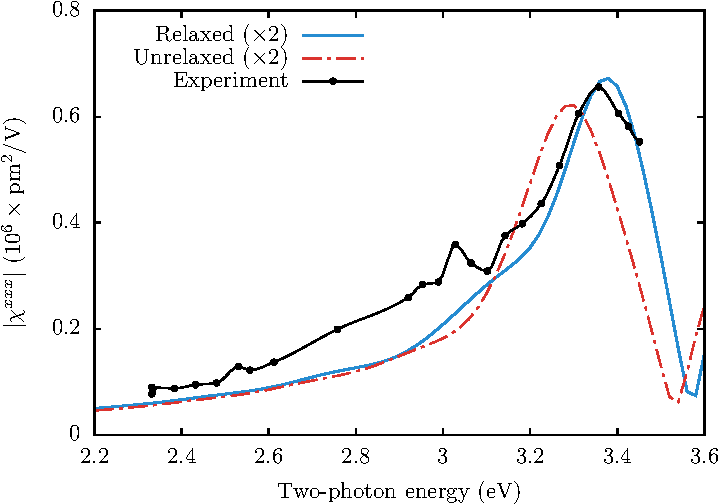
\includegraphics[width=0.6\textwidth]{content/figures/fig-Si1x1-Hofer_Xxxx}
\caption{Comparison of
$\chi^{xxx}$ calculated using relaxed and unrelaxed
atomic positions, with the experimental data presented in Ref.
\cite{hoferAPA96}. The theoretical curves were calculated with a scissors shift
of $\hbar\Delta = 0.7$ eV, and are broadened with $\sigma=0.075\,\text{eV}$.
Experimental data was taken at 80 K.}
\label{fig:Xxxx}
\end{figure}

We can conclude that the most accurate theoretical results are produced by using
relaxed atomic positions for the calculation of $\boldsymbol{\chi}$. Although
this process can be very time consuming for large numbers of atoms, this should
be considered a crucial step. This also further demonstrates that SSHG is very
sensitive to the surface atomic positions. In particular, these results show
that a correct value of the Si-H bond length is not enough to obtain the most
accurate SSHG spectra, and that a full relaxation of the structure is required.
Additionally, it seems that the theory may coincide better with experiments that
are conducted under very low temperature conditions.


%%%%%%%%%%%%%%%%%%%%%%%%%%%%%%%%%%%%%%%%%%%%%%%%%%%%%%%%%%%%%%%%%%%%%%%%%%%%%%%%
%%%%%%%%%%%%%%%%%%%%%%%%%%%%%%%%%%%%%%%%%%%%%%%%%%%%%%%%%%%%%%%%%%%%%%%%%%%%%%%%

\subsection{Comparing the theoretical \texorpdfstring{$\mathcal{R}$}{R} to
experiment}
\label{sec:1x1sshgyield}

All calculations presented from this point on were done using the relaxed atomic
positions described in the the previous section. I will now present the
theoretical SSHG yield for the Si(111)(1$\times$1):H surface compared to
experiments from Refs. \cite{mitchellSS01, mejiaPRB02, bergfeldPRL04}. These
comparisons are good benchmarks to test the complete formalism for calculating
the SSHG yield.

The method of calculation is as follows. I first calculated
$\varepsilon_{b}(\omega)$, $\varepsilon_{\ell}(\omega)$, and then
$\chi^{\mathrm{abc}}$ from Eq. \eqref{eq:chis}. I used these for the Fresnel
factors and in Eqs. \eqref{eq:rpp111}, \eqref{eq:rps111}, and \eqref{eq:rsp111},
and finally, those into Eq. \eqref{eq:mc6} to obtain the theoretical SSHG yield
for different polarizations that can then be compared with the experimental
data. Remember that a scissors shift of $\hbar\Delta = 0.7$ eV is used for all
the $\chi^{\mathrm{abc}}$ components. These were also broadened with a Gaussian
broadening of $\sigma=0.05$ eV, while the calculated ${\mathcal{R}}$ spectra
feature a broadening of $\sigma=0.10$ eV. These values were selected so that the
theoretical calculation best represents the lineshape of the experimental
spectrum.


%%%%%%%%%%%%%%%%%%%%%%%%%%%%%%%%%%%%%%%%%%%%%%%%%%%%%%%%%%%%%%%%%%%%%%%%%%%%%%%%

\subsubsection{Overview of the calculated \texorpdfstring{$\mathcal{R}$}{R}
spectra}\label{sec:1x1R3D}

We will carefully review and compare the calculated $\mathcal{R}$ for each
different polarization case in the following sections. However, I first want to
present a general overview of the theoretical SSHG yield, as I did in Sec.
\ref{sec:2x1R3D}. In Figs. \ref{fig:1x1rP3d} and \ref{fig:1x1rS3d}, I present
these results over a two-photon energy range of 2.5-5 eV. This range corresponds
to the experimental measurements featured in Refs. \cite{mejiaPRB02} and
\cite{bergfeldPRL04}. Note that the SSHG yield drops to zero very rapidly before
for energy values under 3 eV. This is because of the lack of surfaces states due
to the surface H-saturation.

\begin{figure}[h]
\centering
\subbottom[$\mathcal{R}_{pP}$\label{fig:1x1rpp3d}]%
{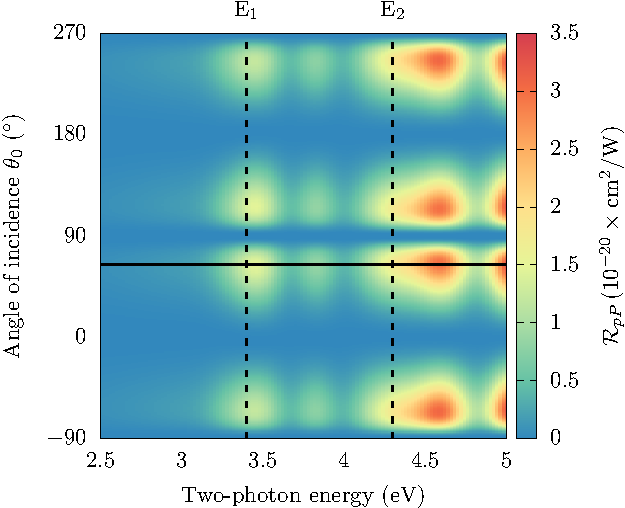
\includegraphics[height=0.39\textwidth]{content/figures/3D-Si1x1-RpP}}\hfill
\subbottom[$\mathcal{R}_{sP}$\label{fig:1x1rsp3d}]%
{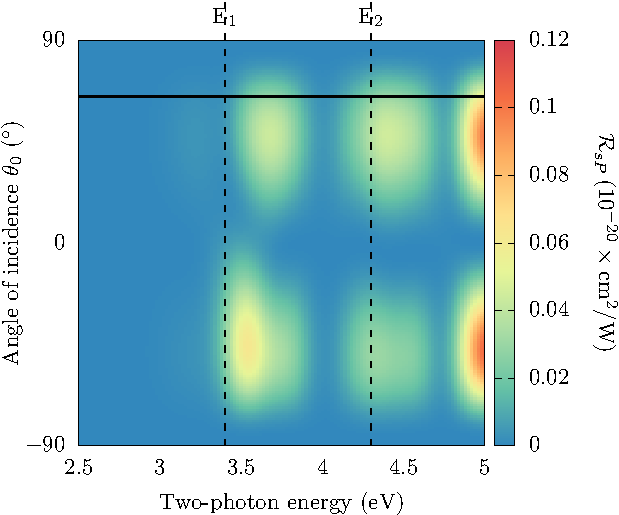
\includegraphics[height=0.39\textwidth]{content/figures/3D-Si1x1-RsP}}
\caption{$\mathcal{R}$ for outgoing $P$ polarization, versus the angle of
incidence ($\theta_{0}$) for the Si(111)(1$\times$1):H surface. A scissors shift
of $\hbar\Delta = 0.7$ eV is applied. The solid line represents $\theta_{0} =
65^{\circ}$, and the dotted lines represent the E$_{1}$ and E$_{2}$ Si critical
points. Both figures consider an azimuthal angle of $\phi = 30^{\circ}$. All
curves are broadened with $\sigma = 0.10$ eV.}
\label{fig:1x1rP3d}
\end{figure}

I have included some helpful markers in these figures. First, the solid black
line represents an angle incidence of $\theta_{0} = 65^{\circ}$. This is one of
two angles that we will consider for the remainder of this chapter; in
particular, this is the angle used in the experiment from Ref. Refs.
\cite{mejiaPRB02}. It is clear that they chose this particular angle to maximize
the $\mathcal{R}_{pP}$ output. Second, the dashed black lines represent the
$E_{1}\sim 3.4$ eV and $E_{2}\sim 4.3$ eV critical points of bulk Si
\cite{yubook}. For the outgoing $P$ polarization in Fig. \ref{fig:1x1rP3d}, we
can see that the calculated SSHG yield does have peaks around those energy
values. We will review this in much further detail below.

\begin{figure}[h]
\centering
\subbottom[$\mathcal{R}_{pS}$\label{fig:1x1rps3d}]%
{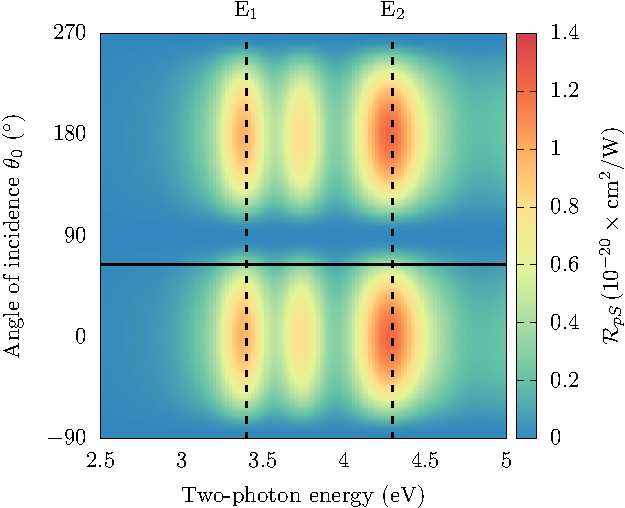
\includegraphics[height=0.39\textwidth]{content/figures/3D-Si1x1-RpS}}\hfill
\subbottom[$\mathcal{R}_{sS}$\label{fig:1x1rss3d}]%
{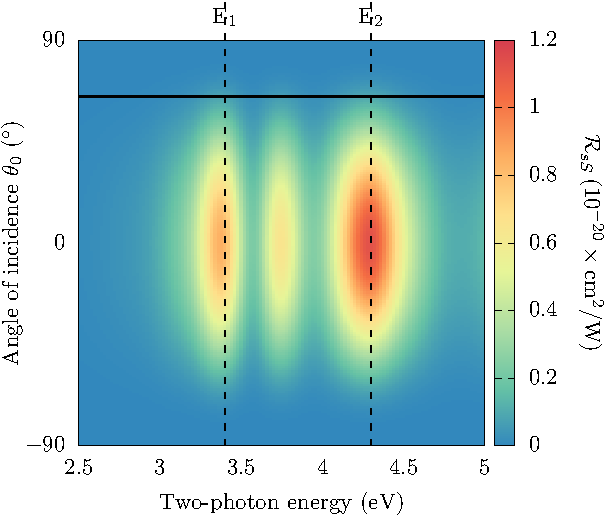
\includegraphics[height=0.39\textwidth]{content/figures/3D-Si1x1-RsS}}
\caption{$\mathcal{R}$ for outgoing $S$ polarized fields, versus the angle of
incidence ($\theta_{0}$) for the Si(111)(1$\times$1):H surface. A scissors shift
of $\hbar\Delta = 0.7$ eV is applied. The solid line represents $\theta_{0} =
65^{\circ}$, and the dotted lines represent the E$_{1}$ and E$_{2}$ Si critical
points. Both figures consider an azimuthal angle of $\phi = 30^{\circ}$. All
curves are broadened with $\sigma = 0.10$ eV.}
\label{fig:1x1rS3d}
\end{figure}

We see similar characteristics, for Fig. \ref{fig:1x1rS3d} with the outgoing $S$
polarization cases. Indeed, the theoretical peak values seem to match quite well
with the critical points. Again, we will review these findings in much more
detail below. Note that I will omit $\mathcal{R}_{sS}$ from this point forward,
as I do not have any experimental data to compare it with.


%%%%%%%%%%%%%%%%%%%%%%%%%%%%%%%%%%%%%%%%%%%%%%%%%%%%%%%%%%%%%%%%%%%%%%%%%%%%%%%%

\subsubsection{\texorpdfstring{$\mathcal{R}_{pP}$}{RpP} ($p$-in, $P$-out)}
\label{sec:1x1RpP}

{\color{red} HERE HERE HERE HERE HERE}

I think the first order of business is to review how the inclusion of multiple reflections affects the 
I think we should first review how the inclusion of multiple reflections affects the produced spectra. 

We consider a Si(111)(1$\times$1):H surface as a test case for the three layer model and to study the effects that multiple reflections have on the SSHG radiation. This surface is well characterized experimentally,\cite{mitchellSS01, mejiaPRB02, bergfeldPRL04} and there has been success in reproducing these experimental results using the three layer model without multiple reflections.\cite{andersonPRB16} The details of the \emph{ab initio} calculation of $\chi^{ijk}$ are not needed for the following discussion, and are left for the reader in Ref. \cite{andersonPRB16}. However, we mention that we apply a scissors shift of 0.7 eV to the theoretical spectra. In a first approximation, this includes the effects of the electronic many-body interactions within the independent particle approach for the \emph{ab initio} calculation. This 0.7 eV value allows the SH resonant peaks to acquire their corresponding energy positions, and is calculated with what is known as a $G_{0}W_{0}$ calculation \cite{andersonPRB16}. We are interested in finding the thickness of the layer $\ell$ where $\chi^{ijk} \ne 0$. For this surface, we found well-converged results for a thickness of $\sim 5$ nm, that is equivalent to 24 atomic sheets of Si along the (111) direction. As this represents only the upper half of the slab, we find it reasonable to choose the thickness of the layer $\ell$ to be between $d\sim 5-10$ nm. This corresponds to a half-slab comprised of 24 to 48 atomic layers to get well-converged values of $\chi^{ijk}$.

We begin our comparisons in Fig. \ref{fig:average}, in which we compare the theoretical results for the SHG radiation with the experimental results from Ref. \cite{mejiaPRB02}. The theoretical curves that include multiple reflections are featured with the average value $\bar{R}^{M}_{i}$, Eq. \eqref{eq:mcave2}, with two values for the total thickness, $d$, and Eqs. \eqref{eq:mc78} and \eqref{eq:rpp111}. We contrast these with the standard three layer model excluding the effects of multiple reflections from Sec. \ref{sec:nomr}. We see that the $E_{2}$ peak is blueshifted by around 0.3 eV, and the yield does not go to zero after 4.75 eV. $\mathcal{R}_{pP}$ is by far the most involved calculation out of the four different polarization cases, since it includes all four nonzero components. In particular, $\chi^{zzz}$ and $\chi^{xxz}$ include out-of-plane incoming fields. These are affected by local field effects that can change both intensity and peak position.\cite{tancognedejean:tel-01235611} Including these effects is computationally very expensive and is beyond the scope of this paper. We speculate that $\mathcal{R}_{pP}$ requires the proper inclusion of these effects in order to accurately describe the experimental peaks.

\begin{figure}[H]
\centering
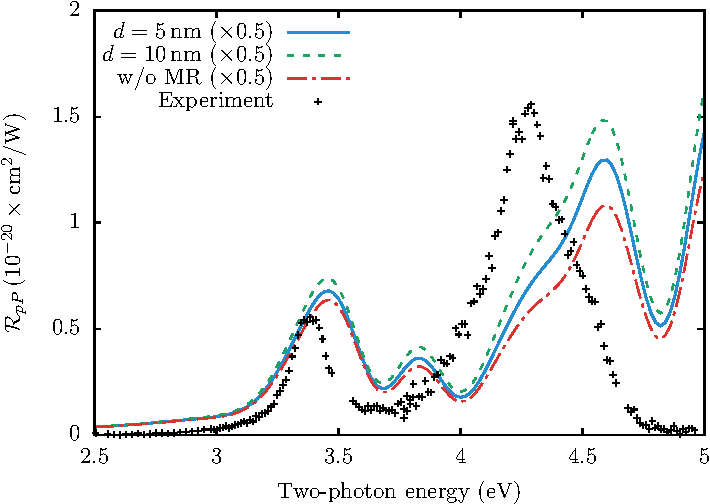
\includegraphics[width=0.5\textwidth]{content/figures/fig-Si1x1-MRthickness}
\caption{Comparison between the three layer model with the effects of multiple reflections for two different values of the total layer thickness $d$, with the standard three layer model without the effects of multiple reflections, and the experimental data from Ref. \cite{mejiaPRB02}. We take $\theta=65^{\circ}$, $\phi=30^{\circ}$, and a scissors value of $\hbar\Delta = 0.7\,\text{eV}$. The $\chi^{ijk}$ components are broadened with $\sigma=0.05\,\text{eV}$, and then $\mathcal{R}_{pP}$ is broadened with $\sigma=0.10\,\text{eV}$.}
\label{fig:average}
\end{figure}

\begin{figure}[H]
\centering
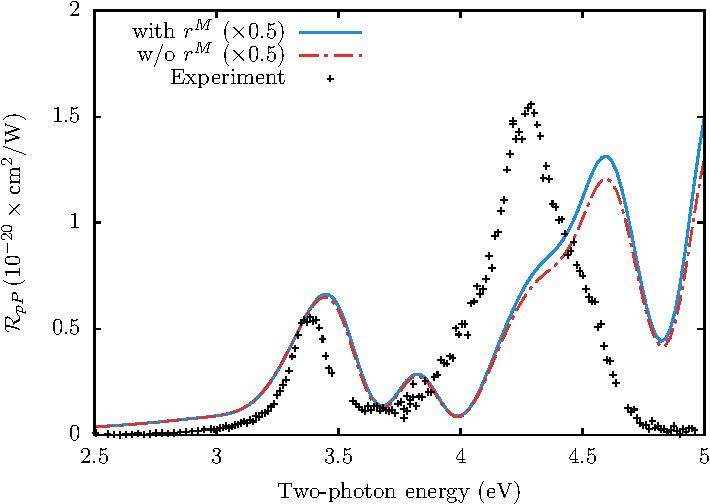
\includegraphics[width=0.5\textwidth]{content/figures/fig-Si1x1-MRno1w}
\caption{Comparison between theoretical models (see Table \ref{tab:models}) and experiment for $\mathcal{R}_{pP}$, for $\theta=65^{\circ}$, and a scissors value of $\hbar\Delta = 0.7\,\text{eV}$. The $\chi^{ijk}$ components are broadened with $\sigma=0.05\,\text{eV}$, and then $\mathcal{R}_{pP}$ is broadened with $\sigma=0.10\,\text{eV}$. Experimental data taken from Ref. \cite{mitchellSS01}, measured at room temperature.}
\label{fig:mr2}
\end{figure}

In Fig. \ref{fig:d2values}, we compare the theoretical results for the SSHG yield with the experimental results from Ref. \cite{mejiaPRB02}. We mention that the experimental results where produced with an angle of incidence of $\theta=65^\circ$, and an azimuthal angle of $\phi=30^\circ$, which eliminates the contribution from $\chi^{xxx}$ from Eq. \eqref{eq:rpp111}. First, we note that the experimental spectrum shows two very well defined resonances which come from electronic transitions from the valence to the conduction bands around the well known $E_{1}\sim 3.4$ eV and $E_{2}\sim 4.3$ eV critical points of Si \cite{yubook}. As can be seen, the theoretical results reproduce the features of the spectrum, although we see that the $E_{2}$ peak is blueshifted by around 0.3 eV. Here we focus on the SSHG yield itself rather than on the physics that lead to such a blueshifted theoretical spectrum. The interested reader can refer to Ref. \cite{andersonPRB16} for those details.

All curves in this figure that include multiple reflections consider $d = 10$ nm. We compare the theoretical SSHG yield for $d_{2} = 0$ nm and $d_{2} = 10$ nm, with the SSHG yield that neglects multiple reflections. When $d_{2} = 0$ nm, we have placed the polarization sheet at the bottom of the layer region. This minimizes the effect of the multiple reflections, and thus the curve is very similar to the three layer model that neglects multiple reflections entirely. When $d_{2} = 10$ nm, the polarization sheet is placed at the top of the layer region. This maximizes the effect of the multiple reflections and therefore leads to the largest yield. We also notice that the average value obtained by using $\bar{R}^{M}_{i}$ (Eq. \eqref{eq:mcave}) is intermediate between $d_{2} = 0$ and $d_{2} = 10$ nm, as expected. This is very similar to selecting $d_{2} = d/2$, which can be interpreted as placing the nonlinear polarization sheet $\mathbf{P}(\mathbf{r},t)$ at the middle of layer $\ell$. It is important to remark that these enhancements are larger for $E_{2}$ than for $E_{1}$. This can be understood from the fact that the corresponding $\lambda_{0}$ for $E_{1}$ is larger than that of $E_{2}$. From Eqs. \eqref{eq:delta0}, \eqref{eq:delta}, and \eqref{mphi}, we see that the phase shifts are larger for $E_{2}$ than for $E_{1}$, producing a larger enhancement of the SSHG yield at $E_{2}$ from the multiple reflections. As the phase shifts grow with $d$, so does the enhancement caused by the multiple reflections. We have verified that the effects of the multiple reflections from the linear field are significantly smaller than those of the SH field. This is clear since the phase shift of Eq. \eqref{mphi} is not only a factor of 2 smaller than that of Eqs. \eqref{eq:delta0} and \eqref{eq:delta}, but also $w_\ell < W_\ell$.

From this figure, it becomes evident that the inclusion of multiple reflections is crucial to obtain a better agreement between the theoretical SSHG yield and the experimental spectrum. This is particularly true for larger energies, such as $E_{2}$, as $\lambda_{0}$ becomes smaller and the multiple reflection effects become more noticeable. The selected value for $d << \lambda_{0}$, that comes naturally from the \emph{ab initio} calculation of $\chi^{ijk}$ is thus very reasonable in order to model a thin surface layer below the vacuum region where the nonlinear SH conversion takes place.

\begin{figure}[H]
\centering
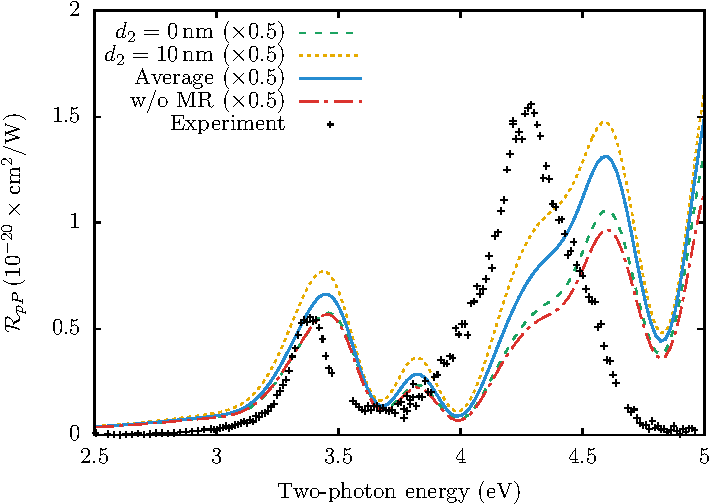
\includegraphics[width=0.5\textwidth]{content/figures/fig-Si1x1-MRdepth}
\caption{Comparison between the three layer model with the effects of multiple reflections for two different values of $d_{2}$, using the average value $\bar{R}^{M}_{i}$ Eq. of Eq. \eqref{eq:mcave2}, the three layer model without the effects of multiple reflections, and the experimental data from Ref. \cite{mejiaPRB02}. All curves that include multiple reflections consider a layer $\ell$ thickness of $d = 10\,\mathrm{nm}$.}
\label{fig:d2values}
\end{figure}


\subsubsection{Calculated \texorpdfstring{$\mathcal{R}_{pP}$}{RpP} compared to
experiment}

I present $\mathcal{R}_{pP}$ compared to experimental data from Ref. \cite{mejiaPRB02} in Fig. \ref{fig:RpP}. Note that peak position for the 3-layer model is similar to experiment with the overall intensity being only two times larger. The E$_{2}$ peak is blueshifted by around 0.3 eV, and the yield does not go to zero after 4.75 eV. The 2-layer-fresnel model produces a spectrum with peak positions that are close to the experiment, but are 20 times more intense. The calculated E$_{2}$ peak is similar, but the E$_{1}$ peak lacks the sharpness present in the experiment. The 2-layer-bulk model is almost identical in lineshape to the 3-layer model, but with eight times less intensity.

From Eq. \eqref{eq:rpp111}, it is clear that $\mathcal{R}_{pP}$ has several $2\omega$ terms that will change between models; this will have a deep effect on the lineshape. Additionally, $\Gamma^{\ell}_{pP}$ also has $\varepsilon_{\ell}(2\omega)$ in the denominator, and so we have a significant difference in both lineshape and intensity between the 2-layer-fresnel and the other two models. Again, as in the previous sections for $\mathcal{R}_{pS}$ and $\mathcal{R}_{sP}$, the 3-layer model is the closest in intensity to the experiment. Additionally, Ref. \cite{dadapPRB97} shows that low temperature measurements of $\mathcal{R}_{pP}$ will blueshift the spectrum away from room temperature measurements such as those shown in Figs. \ref{fig:RpP} and \ref{fig:mitchellRpP}, and towards the theoretical results.

\begin{figure}[H]
\centering 
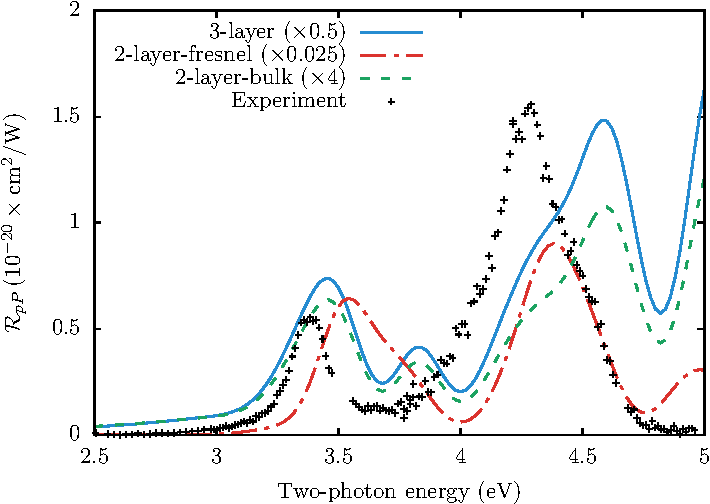
\includegraphics[width=0.5\textwidth]{content/figures/fig-Si1x1-Mejia_RpP}
\caption{Comparison between theoretical models (see Table \ref{tab:models}) and experiment for $\mathcal{R}_{pP}$, for $\theta=65^{\circ}$, and a scissors value of $\hbar\Delta = 0.7\,\text{eV}$. All theoretical curves are broadened with $\sigma=0.10\,\text{eV}$. Experimental data taken from Ref. \cite{mejiaPRB02}, measured at room temperature.}
\label{fig:RpP}
\end{figure}

I'll take this moment to present some auxiliary results from Sec. \ref{sec:scenarios} in Fig. \ref{fig:othermodels}. Refer to Table \ref{tab:models} and Sec. \ref{sec:scenarios}, and note that there are two additional models that we have ignored thus far. The 3-layer-hybrid (Sec. \ref{sec:3-layer-hybrid}) evaluates $\mathcal{P}(2\omega)$ in the thin layer $\ell$ defined by $\epsilon_{ell}$, while the fundamental fields are evaluated in the bulk region defined by $\epsilon_{b}$.

\begin{figure}[H]
\centering 
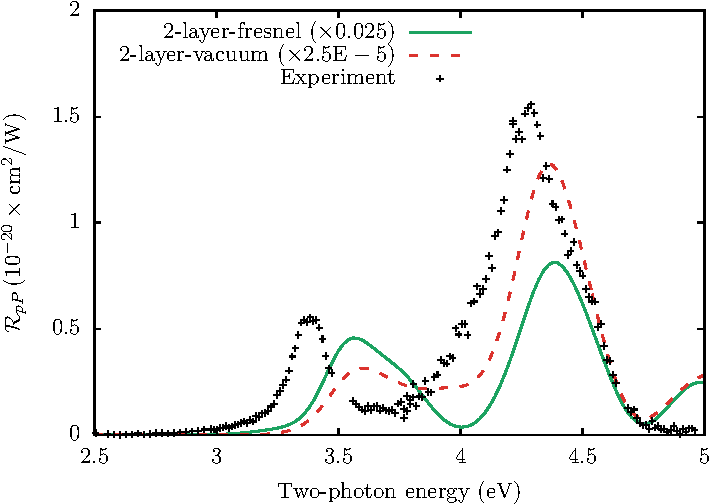
\includegraphics[width=0.5\textwidth]{content/figures/fig-Si1x1-Mejia_RpP_models}
\caption{Other models. \label{fig:othermodels}}
\end{figure}

It is immediately apparent that the 3-layer-hybrid model shares the same lineshape as 3-layer and 2-layer-bulk models, see Fig. \ref{fig:RpP}. This is entirely consistent as $\epsilon_{b}$ and $\epsilon_{\ell}$ differ only in intensity; this model is intermediate in intensity between the other two. The 3-layer model is still closer to experiment, but this is an interesting alternative. On the other hand, the 2-layer-vacuum model has the most extreme intensity difference with the experiment, over 5 orders of magnitude higher. The lineshape reproduces the E$_{2}$ peak quite well, but lacks a sharp E$_{1}$ peak with poor peak position. Clearly, the screening provided by $\epsilon_{b}$ and $\epsilon_{\ell}$ are necessary for accurate results.

Reviewing Eq. \eqref{eq:rpp111}, we see that $\mathcal{R}_{pP}$ is by far the most involved calculation, since it includes all four nonzero components. In particular, $\chi^{zzz}$ and $\chi^{xxz}$ include out-of-plane incoming fields. These are affected by local field effects\cite{tancognedejean:tel-01235611} that reveal the inhomogeneities in the material, which are by far more prevalent perpendicular to the surface than in the surface plane. This can be evidenced for Si, as Reflectance Anisotropy Spectroscopy (RAS) measurements are well described by \emph{ab initio} calculations neglecting local field effects.\cite{palummoPRB99, gaalPRB09} It is therefore expected that the out-of-plane components will be more sensitive to the inclusion of local fields. These will not change the transition energies, only their relative weights of the resonant peaks,\cite{tancognedejean:tel-01235611} but including these effects is challenging to compute,\cite{nicolasPRB15} and beyond the scope of this paper. We speculate that $\mathcal{R}_{pP}$ requires the proper inclusion of these effects in order to accurately describe the experimental peaks.

In Fig. \ref{fig:mitchellRpP}, I compare the theoretical spectra to results from Ref. \cite{mitchellSS01}. The 3-layer model is, as before, close to the experiment in both peak position and intensity. Intensity is almost the same the experimental value. This provides a more compelling argument against the 2-layer-fresnel model than Fig. \ref{fig:RpP}. The 2-layer-fresnel model is 20 times more intense and blueshifted by around 0.1 eV. As mentioned above, this surface is of very high quality with measurements taken shortly after surface preparation. The 2-layer-bulk model is intermediate between the other two models in both intensity and lineshape. Under these conditions, the 3-layer model very accurately reproduces the E$_{1}$ peak over the 2-layer-fresnel and 2-layer-bulk models.

\begin{figure}[H]
\centering
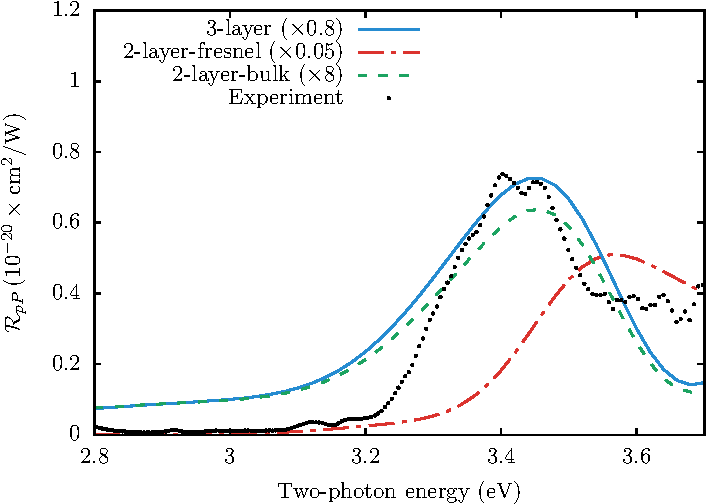
\includegraphics[width=0.5\textwidth]{content/figures/fig-Si1x1-Mitchell_RpP}
\caption{Comparison between theoretical models (see Table \ref{tab:models}) and experiment for $\mathcal{R}_{pP}$, for $\theta=45^{\circ}$, and a scissors value of $\hbar\Delta = 0.7\,\text{eV}$. All theoretical curves are broadened with $\sigma=0.075\,\text{eV}$. Experimental data taken from Ref. \cite{mitchellSS01}, measured at room temperature.}
\label{fig:mitchellRpP}
\end{figure}

Lastly, $GW$ transition energies are needed for linear optics and SHG. Doing a Bethe-Salpeter calculation for SSHG will undoubtedly improve the position and the amplitude of the peaks, but is far beyond current capabilities \cite{puff}. I kept the scissors shift constant throughout these calculations as I want to keep this calculation at the {\em ab initio} level. Remember that the choice of $\hbar\Delta=0.7$ eV for the scissors shift comes from a $GW$ calculation \cite{liPRB10}. As explained in Fig. \ref{fig:improvements}, the lack of surface states causes an almost rigid shift of the spectra by applying the scissors correction. I have checked that it is not possible to have a single scissors value that can reproduce the energy positions of both the E$_{1}$ and the E$_{2}$ peaks. Of course, the experimental temperature at which the spectra is measured should be taken into account in a more complete formulation. However, these calculations are always restricted to $T=0$ K.


%%%%%%%%%%%%%%%%%%%%%%%%%%%%%%%%%%%%%%%%%%%%%%%%%%%%%%%%%%%%%%%%%%%%%%%%%%%%%%%%

\subsubsection{Calculated \texorpdfstring{$\mathcal{R}_{sP}$}{RsP} compared to 
experiment}\label{sec:1x1RsP}

Next, I analyze and compare the calculated $\mathcal{R}_{sP}$ spectra with experimental data from Ref. \cite{mejiaPRB02}. The calculation adheres to the experimental setup by taking an angle of incidence $\theta=65^{\circ}$ and an azimuthal angle $\phi=30^\circ$. As seen in Fig. \ref{fig:RsP}, the overall intensity of $\mathcal{R}_{sP}$ is one order of magnitude lower than $\mathcal{R}_{pS}$. The experimental data is far noisier than in the other cases but the E$_{1}$ and E$_{2}$ peaks are still discernible. As with the previous comparisons, the 3-layer model is the closest match in both intensity and lineshape to the experimental spectrum. It produces a curve that is very close to the experimental intensity with good proportional heights for the calculated E$_{1}$ and E$_{2}$ peaks. In contrast, the 2-layer-fresnel model is 100 times more intense than experiment and produces an enlarged E$_{2}$ peak. The 2-layer-bulk model is ten times smaller with a very similar lineshape to the 3-layer model.

The differences between the 2-layer-fresnel and 2-layer-bulk models are not derived from Eq. \eqref{eq:rsp111}, as the $\varepsilon_{b}(2\omega)$ does not change and the second term vanishes for this azimuthal angle of $\phi = 30$. However, $\Gamma^{\ell}_{sP}$ does cause a significant change in the intensity as there is an $\varepsilon_{\ell}(2\omega)$ term in the denominator. This will become $\varepsilon_{v}(2\omega) = 1$ for the 2-layer-fresnel model, and $\varepsilon_{b}(2\omega)$ in the bulk model. This accounts for the significant difference between the intensity of the two models, while the lineshape remains mostly consistent.

At higher energies, the theoretical curve is blueshifted as compared to the experiment. The best explanation for this is the inclusion of the scissor operator, which does not adequately correct the transitions occurring at these higher energies. A full GW calculation would be well suited for this task, but is well beyond the scope of this work.

\begin{figure}[H]
\centering
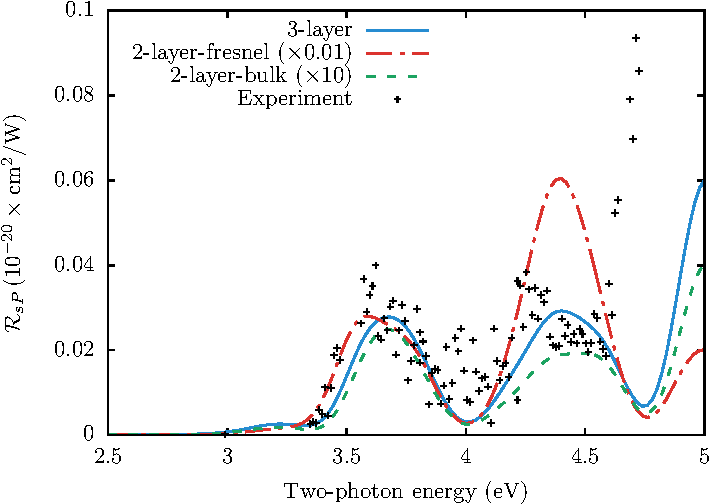
\includegraphics[width=0.5\textwidth]{content/figures/fig-Si1x1-Mejia_RsP}
\caption{Comparison between theoretical models (see Table \ref{tab:models}) and experiment for $\mathcal{R}_{sP}$, for $\theta=65^{\circ}$, and a scissors value of $\hbar\Delta = 0.7\,\text{eV}$. All theoretical curves are broadened with $\sigma=0.075\,\text{eV}$. Experimental data taken from Ref. \cite{mejiaPRB02}, measured at room temperature.}
\label{fig:RsP}
\end{figure}


%%%%%%%%%%%%%%%%%%%%%%%%%%%%%%%%%%%%%%%%%%%%%%%%%%%%%%%%%%%%%%%%%%%%%%%%%%%%%%%%

\subsubsection{Calculated \texorpdfstring{$\mathcal{R}_{pS}$}{RpS} compared to 
experiment}\label{sec:1x1RpS}

I first compare the calculated $\mathcal{R}_{pS}$ spectra with room temperature experimental data from Ref. \cite{mejiaPRB02}. Adhering to the experimental setup, I set an angle of incidence $\theta=65^{\circ}$ and an azimuthal angle of $\phi=30^\circ$ with respect to the $x$-axis. This azimuthal angle maximizes $r_{pS}$, as shown in Eq. \eqref{eq:rps111}. Fig. \ref{fig:RpS}, shows that all three models reproduce the lineshape of the experimental spectrum which includes the peaks corresponding to both the E$_{1}$ (3.4 eV) and E$_{2}$ (4.3 eV) critical points of bulk silicon, and a smaller feature at around 3.8 eV. The calculated E$_{1}$ and E$_{2}$ peaks are redshifted by 0.1 eV and 0.06 eV, respectively, compared with the experimental peaks.

\begin{figure}[H]
\centering
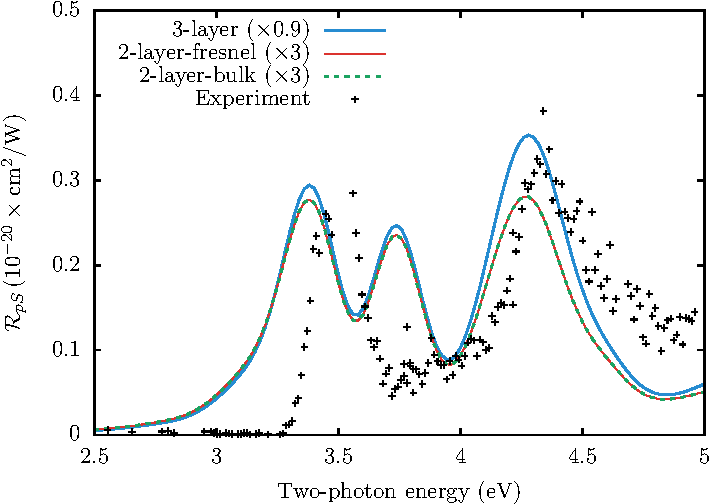
\includegraphics[width=0.5\textwidth]{content/figures/fig-Si1x1-Mejia_RpS}
\caption{Comparison between theoretical models (see Table \ref{tab:models}) and experiment for $\mathcal{R}_{pS}$, for $\theta=65^{\circ}$, and a scissors value of $\hbar\Delta = 0.7\,\text{eV}$. All theoretical curves are broadened with $\sigma=0.075\,\text{eV}$. Experimental data taken from Ref. \cite{mejiaPRB02}, measured at room temperature.}
\label{fig:RpS}
\end{figure}

The main issue to address here is the discrepancy between the intensity of the E$_{1}$ peak. In the theoretical curves, the peaks differ only slightly in overall intensity. Conversely, the experimental E$_{1}$ peak is significantly smaller than the E$_{2}$ peak. This may be due to the effects of oxidation on the surface. Ref. \cite{bergfeldPRL04} features similar data to those of Ref. \cite{mejiaPRB02} but focuses on the effects of surface oxidation. From Ref. \cite{bergfeldPRL04} it is clear that as time passes during the experiment, the surface becomes more oxidized and the E$_{1}$ peak diminishes substantially, as shown by the experimental data taken 5 hours after initial H-termination. This may be enough time to slightly reduce the E$_{1}$ peak intensity, as can be observed here.

In Fig. \ref{fig:mitchellRpS}, I compare the theoretical $\mathcal{R}_{pS}$ with experimental data from Ref. \cite{mitchellSS01}; this data, however, only encompasses the E$_{1}$ peaks, and was obtained at room temperature. This calculation uses an angle of incidence $\theta=45^\circ$ and an azimuthal angle $\phi=30^\circ$ to match the experimental conditions. As in the previous comparison, the E$_{1}$ peak is slightly redshifted compared to experiment. The intensity of the theoretical yield is smaller than the experimental yield for all three models. The measurements presented in Ref. \cite{mitchellSS01} were taken very shortly after the surface had been prepared, and the surface itself was prepared with a high degree of quality and measured at room temperature. Peak position compared to theory is slightly improved under these conditions. As before, the 3-layer model is closer in intensity to the experimental spectrum.

\begin{figure}[H]
\centering
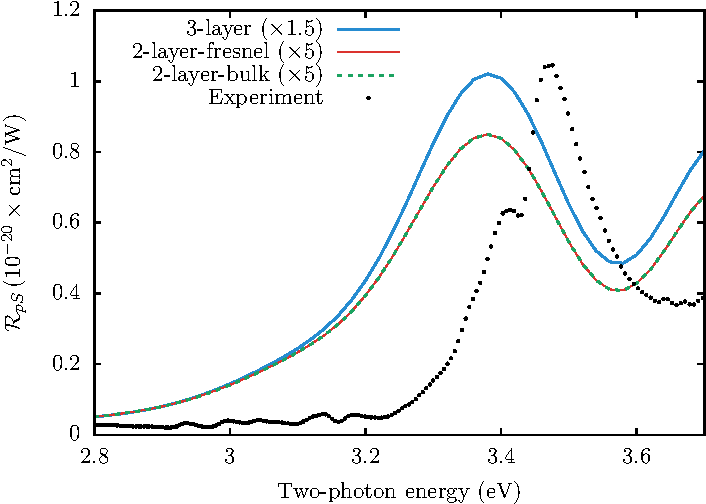
\includegraphics[width=0.5\textwidth]{content/figures/fig-Si1x1-Mitchell_RpS}
\caption{Comparison between theoretical models (see Table \ref{tab:models}) and experiment for $\mathcal{R}_{pS}$, for $\theta=45^\circ$. We use a scissors value of $\hbar\Delta = 0.7\,\text{eV}$. All theoretical curves are broadened with $\sigma=0.075\,\text{eV}$. Experimental data taken from Ref. \cite{mitchellSS01}, measured at room temperature.}
\label{fig:mitchellRpS}
\end{figure}

From Fig. \ref{fig:Xxxx}, I presented that our calculation for $\chi^{xxx}$ coincides with the measurement taken at a low temperature of 80 K. It is well known that temperature causes shifting in the peak position of SSHG spectra \cite{dadapPRB97}. As $\mathcal{R}_{pS}$ only depends on this component (see Eq. \eqref{eq:rps111}), the position of the theoretical peak should be correct in Figs. \ref{fig:RpS} and \ref{fig:mitchellRpS}. Thus, the difference in peak position should stem from the higher temperature at which the experiments were measured.

Both the 2-layer-fresnel and 2-layer-bulk models are identical and roughly four times smaller than the experiment. It is clear from Eq. \eqref{eq:rps111} that $\mathcal{R}_{pS}$ only has $1\omega$ terms ($\varepsilon_{\ell}(\omega)$ and $k_{b}$). For both of these models, the fundamental fields are evaluated in the bulk, which means that the only change to Eq. \eqref{eq:rps111} is that $\varepsilon_{\ell}(\omega) \rightarrow \varepsilon_{b}(\omega)$. Additionally, $\Gamma^{\ell}_{pS}$ also remains identical between the two models and has no $2\omega$ terms in the denominator. Therefore, $r_{pS}$ is identical between these two models. Ultimately, the intensity of the 3-layer model is the closest to the experiment.

Per Eq. \eqref{eq:rps111}, the intensity of $\mathcal{R}_{pS}$ depends only on $\chi^{xxx}$, which is not affected by local field effects \cite{tancognedejean:tel-01235611}. These effects are neglected in this calculation, but $\mathcal{R}_{pS}$ maintains an accurate lineshape and provides a good quantitative description of the experimental SSHG yield. Note that both the calculated and experimental spectra show two-photon resonances at the energies corresponding to the critical point transitions of bulk Si. Note also that the SSHG yield drops rapidly to zero below E$_{1}$, which is consistent with the absence of surface states due to the H saturation on the surface. This observation holds true for all three polarization cases studied for this surface.

Lastly, in Fig. \ref{fig:improvements} I provide an overview of the different levels of approximation proposed in this article. All curves here were calculated using the 3-layer model. The long dashed line depicts the effect of excluding the contribution from the nonlocal part of the pseduopotentials. This is consistent with the results reported in Ref. \cite{andersonPRB15}, where the exclusion of this term increases the intensity of the components of $\boldsymbol{\chi}$ by approximately 15\% to 20\%. Note that the E$_{1}$ peak is larger than the E$_{2}$ peak, contrasting with the experiment, where the E$_{1}$ peak is smaller than E$_{2}$. Lastly, the thin solid line depicts the full calculation with a scissors value of $\hbar\Delta = 0$. The spectrum is almost rigidly redshifted as this H-saturated surface has no electronic surface states \cite{andersonPRB15}. Thus, this demonstrates the importance of including the scissors correction to accurately reproduce the experimental spectrum. In summary, the inclusion of the contribution from the nonlocal part of the pseudopotentials and the scissors operator on top of the 3-layer model produces spectra with a lineshape and intensity that compare favorably with the experimental data.

\begin{figure}[H]
\centering
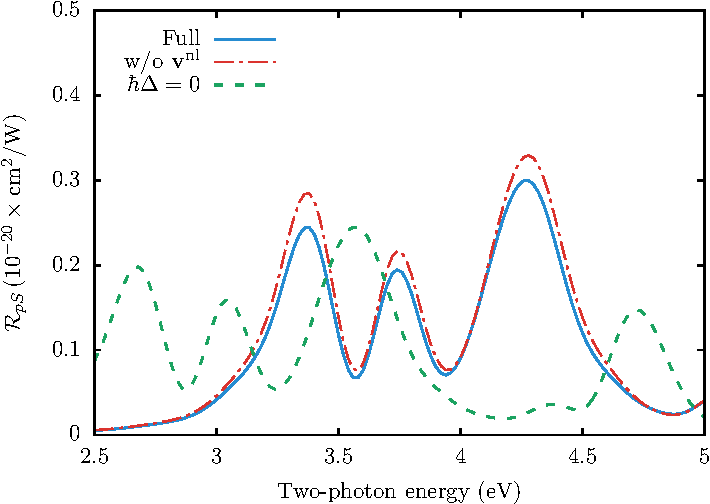
\includegraphics[width=0.5\textwidth]{content/figures/fig-Si1x1-Mejia_RpS_improvements}
\caption{Calculated results for $\mathcal{R}_{pS}$ for the different levels of approximation proposed in this article. All curves were calculated using the 3-layer model. We take $\theta=65^{\circ}$ for this plot. See text for full details. All curves are broadened with $\sigma=0.075\,\text{eV}$.}
\label{fig:improvements}
\end{figure}


\stopcontents[chapters]
